% =====================================================================================
% Quantum Noise Simulation - from density matrices to noisy circuits in CUDA-Q
% Build:  python make_figures.py   (needs cudaq, numpy, scipy, matplotlib; ~5 min on a laptop CPU)
%         latexmk -pdf noise_lecture.tex
% Companion of presentations/qft_source/qft_lecture.tex (same layout and colours).
% =====================================================================================
\documentclass[aspectratio=169,11pt]{beamer}
\usepackage[T1]{fontenc}
\usepackage{lmodern}
\usepackage{amsmath,amssymb}
\usepackage{braket}
\usepackage{graphicx}
\usepackage{booktabs}
\usepackage{array}
\usepackage{tikz}
\usetikzlibrary{arrows.meta,positioning,calc,fit}
\usepackage{quantikz}
\usepackage{listings}
\graphicspath{{figures/}}
% GENERATED by make_figures.py - do not edit
\newcommand{\numpopone}{0.8936}
\newcommand{\numparone}{0.6910}
\newcommand{\numlbone}{0.8601}
\newcommand{\numdistone}{96}
\newcommand{\numtvdone}{0.1064}
\newcommand{\numpopten}{0.3232}
\newcommand{\numparten}{0.0160}
\newcommand{\numdistten}{1165}
\newcommand{\numstimtime}{0.41}
\newcommand{\numreproduced}{identical to the recorded outputs}
\newcommand{\numbfpop}{0.2319}
\newcommand{\numbfpar}{0.1996}
\newcommand{\numpfpop}{1.0000}
\newcommand{\numpfpar}{0.0504}
\newcommand{\numdmfid}{0.9492}
\newcommand{\numdmpur}{0.9013}
\newcommand{\numadfid}{0.7824}
\newcommand{\numadzero}{0.5262}
\newcommand{\numadone}{0.2844}
\newcommand{\numdmcross}{1.3e-15}
\newcommand{\nummirrorgates}{32 + 12}
\newcommand{\nummirrorone}{0.6938}
\newcommand{\nummirrorlb}{0.6426}
\newcommand{\nummirrorzero}{1.000000}
\newcommand{\numblochcheck}{1.1e-16}
\newcommand{\numtonecheck}{8.9e-16}
\newcommand{\numtphi}{133.3}
\newcommand{\numcohsixty}{0.9950}
\newcommand{\numstosixty}{0.0361}
\newcommand{\numpflip}{0.000625}
\newcommand{\numropopideal}{1.0000}
\newcommand{\numropopnoisy}{0.8979}
\newcommand{\numropopmit}{0.9987}
\newcommand{\numrominneg}{-0.0009}
\newcommand{\numzneone}{0.9055}
\newcommand{\numznetwo}{0.8189}
\newcommand{\numznethree}{0.7396}
\newcommand{\numznelin}{0.9921}
\newcommand{\numznequad}{0.9994}
\newcommand{\numzneexp}{1.0021}
\newcommand{\numddfree}{0.149}
\newcommand{\numddecho}{1.000}
\newcommand{\numddtheory}{0.135}
\newcommand{\nummkfree}{0.4420}
\newcommand{\nummkecho}{0.4420}
\newcommand{\nummktheory}{0.4420}
\newcommand{\numqeccheck}{2.6e-16}
\newcommand{\numqecone}{0.000298}
\newcommand{\numqecten}{0.0280}
\newcommand{\numqaoacut}{3.0000}
\newcommand{\numvqeideal}{-3.4141}
\newcommand{\numvqeexact}{-3.4270}
\newcommand{\numqftone}{0.9280}
\newcommand{\numqaoaone}{2.8849}
\newcommand{\numvqeone}{-3.0612}
\newcommand{\numdmten}{122.46}
\newcommand{\numstimfourhundred}{0.04}
\newcommand{\numcudaqversion}{0.16.0}
\newcommand{\numscripttime}{299}


% ---- colours and look (identical to the QFT lecture) ---------------------------------
\definecolor{qblue}{HTML}{2A78D6}
\definecolor{qdark}{HTML}{1C5CAB}
\definecolor{qorange}{HTML}{EB6834}
\definecolor{qaqua}{HTML}{1BAF7A}
\definecolor{qink}{HTML}{0B0B0B}
\definecolor{qgrey}{HTML}{52514E}
\definecolor{qlight}{HTML}{EEF4FC}
\setbeamercolor{structure}{fg=qdark}
\setbeamercolor{frametitle}{fg=qdark}
\setbeamercolor{title}{fg=qdark}
\setbeamercolor{normal text}{fg=qink}
\setbeamercolor{block title}{bg=qblue,fg=white}
\setbeamercolor{block body}{bg=qlight,fg=qink}
\setbeamercolor{block title example}{bg=qaqua,fg=white}
\setbeamercolor{block body example}{bg=qaqua!10,fg=qink}
\setbeamercolor{block title alerted}{bg=qorange,fg=white}
\setbeamercolor{block body alerted}{bg=qorange!10,fg=qink}
\setbeamertemplate{blocks}[rounded][shadow=false]
\setbeamertemplate{navigation symbols}{}
\setbeamertemplate{itemize items}[circle]
\setbeamertemplate{enumerate items}[default]
\setbeamerfont{frametitle}{size=\large,series=\bfseries}
\setbeamertemplate{footline}{%
  \leavevmode\hbox{\begin{beamercolorbox}[wd=\paperwidth,ht=2.4ex,dp=1ex,leftskip=0.4cm,rightskip=0.4cm]{normal text}%
    \color{qgrey}\tiny Quantum Noise Simulation\ \ $\cdot$\ \ \insertsectionhead\hfill\insertframenumber\,/\,\inserttotalframenumber
  \end{beamercolorbox}}}
\newcommand{\hl}[1]{{\color{qorange}\textbf{#1}}}
\newcommand{\key}[1]{{\color{qdark}\textbf{#1}}}
\newcommand{\tagbox}[2]{\tikz[baseline=-0.65ex]\node[fill=#1,text=white,rounded corners=2pt,font=\tiny\bfseries,inner sep=2.2pt]{#2};}
\newcommand{\tagimpl}{\tagbox{qaqua}{IN REPOSITORY}}
\newcommand{\tagtheory}{\tagbox{qgrey}{THEORY ONLY}}
\newcommand{\tagillus}{\tagbox{qorange}{ILLUSTRATIVE EXPERIMENT}}
\newcommand{\E}{\mathcal E}

\lstset{language=Python, basicstyle=\ttfamily\scriptsize, keywordstyle=\color{qdark}\bfseries,
  commentstyle=\color{qgrey}\itshape, stringstyle=\color{qorange}, showstringspaces=false,
  frame=single, rulecolor=\color{qblue!40}, backgroundcolor=\color{qlight}, columns=fullflexible}

\tikzset{
  box/.style={draw=qblue, fill=qlight, rounded corners=3pt, align=center, font=\scriptsize, inner sep=4pt},
  qbox/.style={draw=qorange, fill=qorange!10, rounded corners=3pt, align=center, font=\scriptsize, inner sep=4pt},
  arr/.style={-{Stealth[length=2mm]}, thick, qgrey},
}

\title{Quantum Noise Simulation}
\subtitle{From density matrices and Kraus operators to noisy circuits in CUDA-Q --- explained step by step}
\author{CUDA-Q Quantum Algorithm Benchmarking Suite}
\date{Companion lecture to \texttt{Noise\_Simulation.ipynb}}

\begin{document}

% =====================================================================================
\section{Introduction}
\begin{frame}
  \titlepage
  \centering\small\color{qgrey}
  All results in these slides were computed with NVIDIA CUDA-Q \numcudaqversion{} on a CPU (\texttt{stim}, \texttt{density-matrix-cpu},
  \texttt{qpp-cpu}; no GPU) and checked against independent NumPy calculations. No physical quantum processor was used.
\end{frame}

\begin{frame}{What you will learn today}
  \begin{columns}[T]
    \begin{column}{0.55\textwidth}
      \small
      \begin{enumerate}\itemsep1pt
        \item[1.] \key{Ideal vs noisy} quantum computing: sources of noise, decoherence, fidelity
        \item[2.] \key{Density matrices}, pure and mixed states, \key{quantum channels}, Kraus operators, CPTP maps
        \item[3.] The standard \key{noise channels}: bit, phase and bit-phase flip, depolarizing, amplitude and phase damping
        \item[4.] Hardware noise: two-qubit gates, \key{readout}, $T_1$ and $T_2$, error rates
        \item[5.] \key{Simulating noise} with CUDA-Q: the code of \texttt{Noise\_Simulation.ipynb} line by line, results, benchmarks
        \item[6.] \key{Mitigation and correction}: ZNE, readout mitigation, dynamical decoupling, error correction; hardware outlook
      \end{enumerate}
    \end{column}
    \begin{column}{0.41\textwidth}
      \begin{block}{You only need}
        \small complex numbers, $2\times2$ matrices, basic probability.
      \end{block}
      \begin{alertblock}{Three kinds of statements}
        \scriptsize
        \tagimpl{} code that exists in this repository\\[2pt]
        \tagtheory{} explained, not implemented here\\[2pt]
        \tagillus{} small experiments run for this lecture (\texttt{noise\_source/make\_figures.py})
      \end{alertblock}
    \end{column}
  \end{columns}
\end{frame}

\begin{frame}[label=fRepo]{What this repository actually contains}
  \footnotesize
  \begin{center}
  \resizebox{\linewidth}{!}{%
  \begin{tabular}{lll}
    \toprule \textbf{Topic} & \textbf{Status} & \textbf{Where}\\ \midrule
    GHZ and mirror circuits; 4 noise models after every gate & \tagimpl & \texttt{Noise\_Simulation.ipynb}\\
    \texttt{stim}, density-matrix and GPU-trajectory methods & \tagimpl & \dots\ + \texttt{common\_utils.py}\\
    population, parity, Hellinger, TVD, fidelity, purity, $(1-p)^G$ & \tagimpl & \texttt{Noise\_Simulation.ipynb}\\ \midrule
    channels on the Bloch sphere, $T_1$/$T_2$, coherent and readout errors, & \tagillus & \texttt{make\_figures.py}\\
    \quad ZNE, DD, bit-flip code, noisy QFT/QAOA/VQE, simulation cost & & \\ \midrule
    readout noise in the notebook, RB, surface codes, hardware runs & \tagtheory & ---\\ \bottomrule
  \end{tabular}}
  \end{center}
  \small No GPU, multi-GPU or quantum-hardware run was performed: the trajectory (GPU) path of the notebook exists but was not executed.
  Qiskit/Aer or other simulators are not used anywhere in the repository.
\end{frame}

% =====================================================================================
\section{Part 1: Ideal and noisy quantum computing}
\begin{frame}[label=fIdeal]{Ideal quantum computing}
  \begin{columns}[T]
    \begin{column}{0.52\textwidth}
      \small
      An ideal quantum computer
      \begin{itemize}\itemsep1pt
        \item starts in a perfect state $\ket{0\cdots0}$
        \item applies perfect unitary gates: $\ket\psi \mapsto U\ket\psi$, $U^\dagger U = I$
        \item stays in a \key{pure} state at all times
        \item measures perfectly: $P(x) = |\braket{x|\psi}|^2$ (Born rule)
      \end{itemize}
      Only \key{shot noise} remains: probabilities are estimated from a finite number of runs, with error $\approx\sqrt{P(1-P)/S}$.
    \end{column}
    \begin{column}{0.44\textwidth}
      \begin{exampleblock}{The GHZ state of the notebook}
        \centering
        \begin{quantikz}[row sep=0.18cm, column sep=0.35cm]
          \lstick{$\ket0$} & \gate{H} & \ctrl{1} & \qw & \meter{}\\
          \lstick{$\ket0$} & \qw & \targ{} & \ctrl{1} & \meter{}\\
          \lstick{$\ket0$} & \qw & \qw & \targ{} & \meter{}
        \end{quantikz}\\[2pt]
        \scriptsize $\ket{\mathrm{GHZ}} = \frac{1}{\sqrt2}(\ket{0\cdots0} + \ket{1\cdots1})$: ideally only two outcomes, $50\,\%$ each, and
        parity $\langle X^{\otimes N}\rangle = 1$.
      \end{exampleblock}
    \end{column}
  \end{columns}
\end{frame}

\begin{frame}[label=fIdealNoisy]{Ideal versus noisy circuits \tagimpl}
  \begin{columns}[T]
    \begin{column}{0.58\textwidth}
      \centering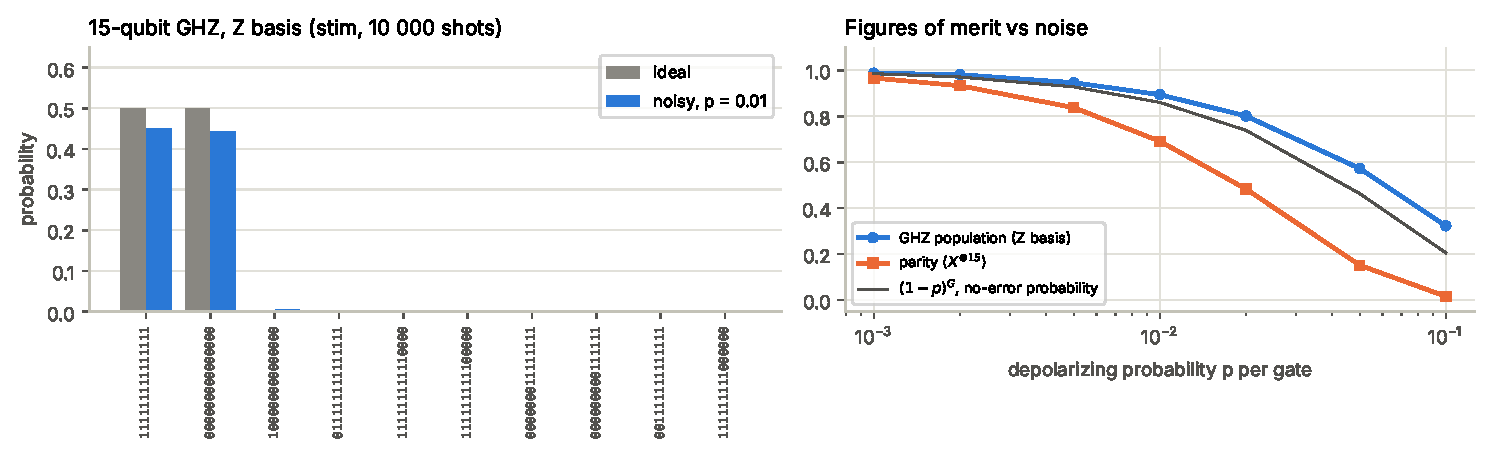
\includegraphics[width=\textwidth]{ghz_sweep}
    \end{column}
    \begin{column}{0.38\textwidth}
      \small
      Notebook default: 15-qubit GHZ, depolarizing noise after every gate, \texttt{stim}, 10\,000 shots.
      \begin{itemize}\itemsep1pt\scriptsize
        \item ideal: 2 outcomes; at $p = 0.01$: \numdistone{} outcomes, population \numpopone
        \item the parity $\langle X^{\otimes15}\rangle$ falls faster: \numparone
        \item at $p = 0.1$: population \numpopten, parity \numparten, \numdistten{} outcomes
      \end{itemize}
      \scriptsize Re-executed for these slides: \numreproduced.
    \end{column}
  \end{columns}
\end{frame}

\begin{frame}[label=fSources]{Sources of quantum noise}
  \footnotesize
  \begin{center}
  \resizebox{\linewidth}{!}{%
  \begin{tabular}{llll}
    \toprule \textbf{source} & \textbf{example} & \textbf{category} & \textbf{typical model}\\ \midrule
    control imperfections & pulse amplitude 1\,\% too large & coherent error & extra unitary $e^{-i\varepsilon H}$\\
    environment: energy exchange & photon emission, two-level defects & decoherence ($T_1$) & amplitude damping\\
    environment: fluctuating fields & flux / charge noise, nuclear spins & decoherence ($T_2$, $T_\varphi$) & phase damping, random phases\\
    gate implementation & finite fidelity of two-qubit gates & stochastic gate noise & depolarizing / Pauli channels\\
    crosstalk & neighbour gates rotate idle qubits & correlated coherent error & multi-qubit unitaries\\
    leakage & excitation to $\ket2$ in transmons & outside the qubit space & qutrit models\\
    state preparation and measurement & thermal population, misassigned outcomes & SPAM / readout error & confusion matrix\\ \bottomrule
  \end{tabular}}
  \end{center}
  \small The notebook models the fourth row (Pauli channels) and amplitude damping. Crosstalk, leakage, drift and readout errors are
  \emph{not} modelled --- a central difference between simulated and real hardware noise.
\end{frame}

\begin{frame}[label=fDecoh]{Decoherence: entanglement with the environment}
  \begin{columns}[T]
    \begin{column}{0.52\textwidth}
      \small
      A qubit interacts with its environment $E$:
      \[ (\alpha\ket0 + \beta\ket1)\ket{e} \mapsto \alpha\ket0\ket{e_0} + \beta\ket1\ket{e_1}. \]
      Tracing out $E$:
      \[ \rho = \begin{pmatrix}|\alpha|^2 & \alpha\beta^*\braket{e_1|e_0}\\ \alpha^*\beta\braket{e_0|e_1} & |\beta|^2\end{pmatrix}. \]
      The coherence shrinks by $|\braket{e_0|e_1}| \le 1$: the environment ``learned'' which state the qubit is in.
    \end{column}
    \begin{column}{0.44\textwidth}
      \begin{exampleblock}{Two worked examples}
        \scriptsize
        \textbf{Entanglement}: $\sqrt{0.8}\ket{00} + \sqrt{0.2}\ket{11}$ gives $\rho_A = \operatorname{diag}(0.8, 0.2)$, purity $0.68$, although the
        global state is pure.\\[3pt]
        \textbf{Random phase}: $\frac{1}{\sqrt2}(\ket0 + e^{i\varphi}\ket1)$, $\varphi$ uniform in $[-\frac\pi2, \frac\pi2]$: $\overline{\langle X\rangle} = \frac2\pi = 0.64$.
      \end{exampleblock}
      \begin{block}{Decoherence vs.\ coherent error}
        \scriptsize Decoherence makes the state \emph{mixed} (information leaks out); a coherent error keeps it pure but wrong.
      \end{block}
    \end{column}
  \end{columns}
\end{frame}

\begin{frame}[label=fFid]{Quantum state fidelity}
  \begin{columns}[T]
    \begin{column}{0.52\textwidth}
      \small
      \begin{itemize}\itemsep2pt
        \item pure vs.\ pure: $F = |\braket{\psi|\phi}|^2$
        \item pure target, mixed state: $F = \braket{\psi|\rho|\psi}$ --- used by the notebook
        \item general: $F(\rho, \sigma) = \big(\operatorname{Tr}\sqrt{\sqrt\rho\,\sigma\sqrt\rho}\big)^2$ (some texts omit the square)
        \item GHZ: $F = \frac12(\rho_{0\cdots0,0\cdots0} + \rho_{1\cdots1,1\cdots1}) + \operatorname{Re}\rho_{0\cdots0,1\cdots1}$ --- needs the coherence
      \end{itemize}
    \end{column}
    \begin{column}{0.44\textwidth}
      \begin{exampleblock}{Numerical examples}
        \scriptsize
        $\rho = 0.8\ket+\!\bra+ + 0.2\frac I2$: $F = 0.8 + 0.1 = 0.9$.\\[2pt]
        Tomography $\rho = \begin{psmallmatrix}0.55&0.35\\0.35&0.45\end{psmallmatrix}$, target $\ket+$: $F = \frac{1 + r_x}{2} = 0.85$.\\[2pt]
        6-qubit GHZ, depolarizing $p = 0.01$ after every gate (density matrix, notebook model): $F = \numdmfid$, purity $\numdmpur$.
      \end{exampleblock}
      \scriptsize Classical counterpart (from samples): Hellinger fidelity $F_H = (\sum_x\sqrt{p_xq_x})^2$.
    \end{column}
  \end{columns}
\end{frame}

\begin{frame}[label=fImperfect]{Quantum gates and imperfect operations \tagillus}
  \begin{columns}[T]
    \begin{column}{0.48\textwidth}
      \small
      \key{Coherent error}: $X$ implemented as $R_X(\pi + \varepsilon)$: $P(\text{error}) = \sin^2\frac\varepsilon2$ ($\varepsilon = 0.1$: $0.0025$).\\[3pt]
      Repeated $n$ times, the angles \emph{add}: $\sin^2\frac{n\varepsilon}{2}$ --- grows like $n^2$.\\[3pt]
      \key{Stochastic error} with the same per-gate probability $p = \sin^2\frac\varepsilon2$: $\frac12[1 - (1-2p)^n] \approx np$ --- grows like $n$.
    \end{column}
    \begin{column}{0.48\textwidth}
      \centering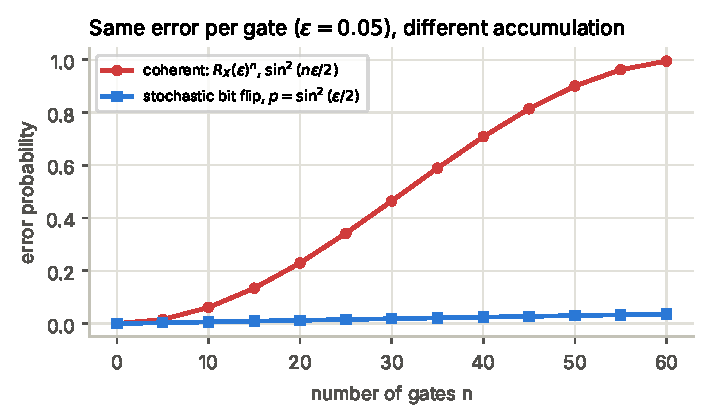
\includegraphics[width=\textwidth]{coherent_vs_stochastic}\\
      {\scriptsize $\varepsilon = 0.05$, $n = 60$: coherent \numcohsixty, stochastic \numstosixty{} (CUDA-Q).}
    \end{column}
  \end{columns}
  \small Same average gate fidelity, wildly different circuits: coherent errors are the most dangerous. Pauli twirling (slide ``Twirling'') converts them
  into the stochastic Pauli noise that the notebook simulates.
\end{frame}

% =====================================================================================
\section{Part 2: Density matrices and quantum channels}
\begin{frame}[label=fDM]{Density matrices}
  \begin{columns}[T]
    \begin{column}{0.52\textwidth}
      \small
      An ensemble ``$\ket{\psi_i}$ with probability $p_i$'' is described by
      \[ \rho = \sum_ip_i\ket{\psi_i}\!\bra{\psi_i}. \]
      Properties: $\rho = \rho^\dagger$, $\operatorname{Tr}\rho = 1$, $\rho \ge 0$.
      \begin{itemize}\itemsep1pt
        \item probabilities: $P(k) = \rho_{kk}$; expectation values $\langle M\rangle = \operatorname{Tr}(\rho M)$
        \item gates: $\rho \mapsto U\rho U^\dagger$
        \item $N$ qubits: $2^N\times2^N$, i.e.\ $4^N$ numbers ($16\cdot4^N$ bytes)
      \end{itemize}
    \end{column}
    \begin{column}{0.44\textwidth}
      \begin{exampleblock}{Examples}
        \scriptsize
        $\frac{1}{\sqrt2}(\ket0 + i\ket1) \mapsto \frac12\begin{psmallmatrix}1 & -i\\ i & 1\end{psmallmatrix}$ (pure).\\[3pt]
        $\begin{psmallmatrix}0.6 & 0.5\\ 0.5 & 0.4\end{psmallmatrix}$ is \emph{not} a state: $\det = -0.01 < 0$.\\[3pt]
        Two independent qubits $\operatorname{diag}(0.9, 0.1)\otimes\operatorname{diag}(0.8, 0.2)$: $P(\text{equal}) = 0.72 + 0.02 = 0.74$.
      \end{exampleblock}
    \end{column}
  \end{columns}
\end{frame}

\begin{frame}[label=fPure]{Pure and mixed states on the Bloch ball}
  \begin{columns}[T]
    \begin{column}{0.40\textwidth}
      \centering
      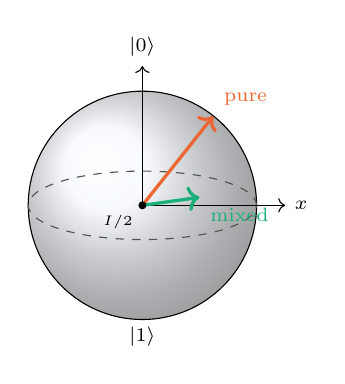
\begin{tikzpicture}[scale=1.45]
        \shade[ball color=qlight, opacity=0.6] (0,0) circle (1);
        \draw (0,0) circle (1); \draw[dashed, qgrey] (0,0) ellipse (1 and 0.3);
        \draw[->] (0,0) -- (0,1.22) node[above, font=\scriptsize]{$\ket0$};
        \draw[->] (0,0) -- (1.25,0) node[right, font=\scriptsize]{$x$};
        \node[font=\scriptsize] at (0,-1.15) {$\ket1$};
        \draw[->, very thick, qorange] (0,0) -- (0.62,0.78) node[above right, font=\scriptsize]{pure};
        \draw[->, very thick, qaqua] (0,0) -- (0.5,0.07) node[below right, font=\scriptsize]{mixed};
        \fill (0,0) circle (1pt) node[below left, font=\tiny]{$I/2$};
      \end{tikzpicture}
    \end{column}
    \begin{column}{0.56\textwidth}
      \small
      $\rho = \frac12(I + r_xX + r_yY + r_zZ)$, $|\vec r| \le 1$.
      \begin{itemize}\itemsep1pt
        \item pure $\Leftrightarrow$ $|\vec r| = 1$ $\Leftrightarrow$ $\operatorname{Tr}\rho^2 = 1$; mixed $\Leftrightarrow$ inside the ball
        \item $\operatorname{Tr}\rho^2 = \frac{1 + |\vec r|^2}{2}$; eigenvalues $\frac{1 \pm |\vec r|}{2}$
        \item maximally mixed $I/2$ at the centre; $N$ qubits: purity $\ge 2^{-N}$
      \end{itemize}
      \begin{exampleblock}{Worked example}
        \scriptsize $\rho = \begin{psmallmatrix}0.7&0.3\\0.3&0.3\end{psmallmatrix}$: $\vec r = (0.6, 0, 0.4)$, purity $0.76$, eigenvalues $0.861$, $0.139$.
        Noise channels act on $\vec r$ as \key{affine maps} that shrink (and may shift) the ball.
      \end{exampleblock}
    \end{column}
  \end{columns}
\end{frame}

\begin{frame}[label=fChan]{Quantum channels and Kraus operators}
  \begin{columns}[T]
    \begin{column}{0.52\textwidth}
      \small
      Every physical noise process on a system is a \key{quantum channel} with a \key{Kraus representation}
      \[ \E(\rho) = \sum_kK_k\rho K_k^\dagger,\qquad \sum_kK_k^\dagger K_k = I. \]
      Interpretation: with probability $p_k = \operatorname{Tr}(K_k\rho K_k^\dagger)$ ``event $k$'' happens and the state becomes $K_k\rho K_k^\dagger/p_k$.
      \begin{itemize}\itemsep0pt\scriptsize
        \item it arises from a unitary on system + environment, followed by tracing out the environment (Stinespring)
        \item a $d$-dimensional channel needs at most $d^2$ Kraus operators
      \end{itemize}
    \end{column}
    \begin{column}{0.44\textwidth}
      \begin{exampleblock}{Worked example: completeness}
        \scriptsize $K_0 = \operatorname{diag}(1, 0.8)$, $K_1 = b\ket0\!\bra1$: $K_0^\dagger K_0 + K_1^\dagger K_1 = \operatorname{diag}(1, 0.64 + b^2)$, so $b = 0.6$
        --- amplitude damping with $\gamma = 0.36$.
      \end{exampleblock}
      \begin{exampleblock}{Worked example: applying a channel}
        \scriptsize Bit flip $p = 0.2$ on $\begin{psmallmatrix}0.9&0.3\\0.3&0.1\end{psmallmatrix}$: $0.8\rho + 0.2X\rho X = \begin{psmallmatrix}0.74&0.30\\0.30&0.26\end{psmallmatrix}$.
      \end{exampleblock}
    \end{column}
  \end{columns}
\end{frame}

\begin{frame}[label=fCPTP]{Completely positive trace-preserving (CPTP) maps}
  \begin{columns}[T]
    \begin{column}{0.52\textwidth}
      \small
      A map $\E$ is a valid quantum operation iff it is
      \begin{itemize}\itemsep1pt
        \item \key{linear},
        \item \key{trace preserving}: $\operatorname{Tr}\E(\rho) = \operatorname{Tr}\rho$ $\Leftrightarrow$ $\sum K^\dagger K = I$,
        \item \key{completely positive}: $(\E\otimes\mathrm{id})(\rho_{AB}) \ge 0$ for every state of system $+$ any ancilla.
      \end{itemize}
      Kraus form $\Rightarrow$ CP automatically. The transpose $\rho \mapsto \rho^{\mathsf T}$ is positive but \emph{not} CP --- not physical.\\[3pt]
      \key{Choi state}: $J(\E) = (\E\otimes\mathrm{id})(\ket{\Phi^+}\!\bra{\Phi^+})$; $\E$ is CP iff $J \ge 0$; the process fidelity is $\braket{\Phi^+|J|\Phi^+}$.
    \end{column}
    \begin{column}{0.44\textwidth}
      \begin{block}{Kraus operators are not unique}
        \scriptsize $\{\sqrt{1-p}I, \sqrt pZ\}$ (phase flip) and $\{\operatorname{diag}(1, \sqrt{1-\lambda}), \operatorname{diag}(0, \sqrt\lambda)\}$ (phase damping) are the
        same channel when $1 - 2p = \sqrt{1-\lambda}$, e.g.\ $\lambda = 0.36 \leftrightarrow p = 0.1$.
      \end{block}
      \begin{alertblock}{Check}
        \scriptsize $\{I, \sqrt{0.1}X\}$: $\sum K^\dagger K = 1.1I$ --- not trace preserving.
        $\{\sqrt{0.7}I, \sqrt{0.3}Y\}$ --- valid (bit-phase flip).
      \end{alertblock}
    \end{column}
  \end{columns}
\end{frame}

% =====================================================================================
\section{Part 3: The standard noise channels}
\begin{frame}[label=fBF]{Bit-flip channel}
  \begin{columns}[T]
    \begin{column}{0.52\textwidth}
      \small
      \key{Physics}: an unwanted $X$ (e.g.\ a spurious $\pi$ pulse) with probability $p$.\\
      \key{Kraus}: $K_0 = \sqrt{1-p}\,I$, $K_1 = \sqrt p\,X$.
      \[ \E(\rho) = (1-p)\rho + pX\rho X, \]
      \[ (r_x, r_y, r_z) \mapsto (r_x,\ (1-2p)r_y,\ (1-2p)r_z). \]
      \key{Effect}: the ball shrinks towards the $x$-axis; $\ket\pm$ are immune.\\
      \key{Example}: $\ket0$, $p = 0.1$: $\rho = \operatorname{diag}(0.9, 0.1)$, $P(1) = 0.1$, purity $0.82$.
    \end{column}
    \begin{column}{0.44\textwidth}
      \key{\small Circuit level} {\scriptsize ($X_p$: $X$ with probability $p$)}\\[2pt]
      \centering
      \begin{quantikz}[row sep=0.2cm, column sep=0.35cm]
        \lstick{$\ket\psi$} & \gate{U} & \gate[style={fill=qorange!15}]{X_p} & \meter{}
      \end{quantikz}\\[4pt]
      \scriptsize CUDA-Q: \texttt{cudaq.BitFlipChannel(p)}. In the notebook (\texttt{bit\_flip}): after every \texttt{h}, \texttt{x}, \texttt{ry},
      \texttt{rz}, and independently on both qubits after every CNOT (\texttt{Pauli2}: $IX$, $XI$ with $p(1-p)$, $XX$ with $p^2$).
      \tagimpl
    \end{column}
  \end{columns}
\end{frame}

\begin{frame}[label=fPF]{Phase-flip channel}
  \begin{columns}[T]
    \begin{column}{0.52\textwidth}
      \small
      \key{Physics}: a random phase kick $Z$ (dephasing).\\
      \key{Kraus}: $\sqrt{1-p}\,I$, $\sqrt p\,Z$.
      \[ \E(\rho) = \begin{pmatrix}\rho_{00} & (1-2p)\rho_{01}\\ (1-2p)\rho_{10} & \rho_{11}\end{pmatrix}. \]
      \key{Effect}: $(r_x, r_y, r_z) \mapsto ((1-2p)r_x, (1-2p)r_y, r_z)$; populations unchanged.\\
      \key{Example}: $\ket+$, $p = 0.1$: $\langle X\rangle = 0.8$, $P(+) = 0.9$; $p = \frac12$ destroys all coherence, $p = 1$ is just a $Z$ gate.
    \end{column}
    \begin{column}{0.44\textwidth}
      \begin{alertblock}{Invisible in the $Z$ basis}
        \scriptsize 15-qubit GHZ with phase-flip noise $p = 0.05$ (\texttt{stim}): population \numpfpop, but $X$-basis parity \numpfpar.
        One $Z$ error maps $\ket{0\cdots0} + \ket{1\cdots1} \to \ket{0\cdots0} - \ket{1\cdots1}$.
      \end{alertblock}
      \scriptsize CUDA-Q: \texttt{cudaq.PhaseFlipChannel(p)}; notebook: \texttt{phase\_flip} (\texttt{Pauli2}: $IZ$, $ZI$, $ZZ$). \tagimpl
    \end{column}
  \end{columns}
\end{frame}

\begin{frame}[label=fYF]{Bit-phase-flip channel}
  \begin{columns}[T]
    \begin{column}{0.52\textwidth}
      \small
      \key{Physics}: both a flip and a phase error, $Y = iXZ$.\\
      \key{Kraus}: $\sqrt{1-p}\,I$, $\sqrt p\,Y$.
      \[ (r_x, r_y, r_z) \mapsto ((1-2p)r_x,\ r_y,\ (1-2p)r_z). \]
      \key{Effect}: shrink towards the $y$-axis; it flips $Z$ outcomes \emph{and} the sign of $\langle X\rangle$.\\
      \key{Example}: $p = 0.3$ on $\ket0$: $\langle Z\rangle = 0.4$; on $\ket+$: $\langle X\rangle = 0.4$ (measured with CUDA-Q \texttt{YError}).
    \end{column}
    \begin{column}{0.44\textwidth}
      \begin{block}{Pauli channels in general}
        \scriptsize $\E(\rho) = p_I\rho + p_XX\rho X + p_YY\rho Y + p_ZZ\rho Z$ maps $r_k \mapsto (1 - 2(p_j + p_l))r_k$ ($j, l$ the other two Paulis).
        Bit, phase, bit-phase flip and depolarizing are special cases. \tagtheory{} for the notebook (library: \texttt{cudaq.YError}, \texttt{Pauli1}).
      \end{block}
    \end{column}
  \end{columns}
\end{frame}

\begin{frame}[label=fDep]{Depolarizing channel}
  \begin{columns}[T]
    \begin{column}{0.52\textwidth}
      \small
      \key{Physics}: an unknown random Pauli error --- the standard ``average'' gate error.\\
      \key{Kraus} (CUDA-Q): $\sqrt{1-p}\,I$, $\sqrt{p/3}\,X$, $\sqrt{p/3}\,Y$, $\sqrt{p/3}\,Z$.
      \begin{align*} \E(\rho) &= (1-p)\rho + \tfrac p3(X\rho X + Y\rho Y + Z\rho Z)\\ &= (1-\lambda)\rho + \lambda\tfrac I2,\qquad \lambda = \tfrac{4p}{3}. \end{align*}
      \key{Effect}: $\vec r \mapsto (1 - \frac{4p}{3})\vec r$ --- isotropic shrink.\\
      \key{Example}: $p = 0.03$ on $\ket0$: $P(1) = \frac{2p}{3} = 0.02$. Measured: \texttt{DepolarizationChannel(0.3)} on $\ket0$ gives $\langle Z\rangle = 0.6$.
    \end{column}
    \begin{column}{0.44\textwidth}
      \begin{block}{Two-qubit version (\texttt{Depolarization2})}
        \scriptsize $\sqrt{1-p}\,II$ and the 15 other two-qubit Paulis with probability $p/15$ each. Probability that the control's $Z$ outcome flips:
        $8p/15$ ($X$ or $Y$ on the control).
      \end{block}
      \begin{alertblock}{Conventions differ}
        \scriptsize Some texts write $(1-p)\rho + pI/2$; then CUDA-Q's $p$ equals $\frac34$ of theirs. Always check the Kraus operators.
      \end{alertblock}
      \scriptsize Default noise of the notebook. \tagimpl
    \end{column}
  \end{columns}
\end{frame}

\begin{frame}[label=fAD]{Amplitude damping (energy relaxation, $T_1$)}
  \begin{columns}[T]
    \begin{column}{0.52\textwidth}
      \small
      \key{Physics}: $\ket1$ decays to $\ket0$ by emitting energy.\\
      \key{Kraus}: $K_0 = \begin{psmallmatrix}1&0\\0&\sqrt{1-\gamma}\end{psmallmatrix}$ (no jump), $K_1 = \begin{psmallmatrix}0&\sqrt\gamma\\0&0\end{psmallmatrix}$ (jump).
      \[ \E(\rho) = \begin{pmatrix}\rho_{00} + \gamma\rho_{11} & \sqrt{1-\gamma}\,\rho_{01}\\ \sqrt{1-\gamma}\,\rho_{10} & (1-\gamma)\rho_{11}\end{pmatrix}. \]
      \key{Effect}: $r_{x,y} \mapsto \sqrt{1-\gamma}\,r_{x,y}$, $r_z \mapsto \gamma + (1-\gamma)r_z$ --- \hl{non-unital}: $I/2$ is not a fixed point.
    \end{column}
    \begin{column}{0.44\textwidth}
      \begin{exampleblock}{Worked example}
        \scriptsize $\ket+$, $\gamma = 0.36$: $\begin{psmallmatrix}0.68 & 0.40\\ 0.40 & 0.32\end{psmallmatrix}$.\\
        Notebook model on a 6-qubit GHZ, $\gamma = 0.05$ (density matrix): $P(0\cdots0) = \numadzero$, $P(1\cdots1) = \numadone$ --- outcomes biased towards 0;
        fidelity \numadfid.
      \end{exampleblock}
      \scriptsize CUDA-Q: \texttt{AmplitudeDampingChannel}; on CNOTs the notebook uses a 4-operator \texttt{KrausChannel} ($K_i\otimes K_j$). Not a Pauli channel: no \texttt{stim}. \tagimpl
    \end{column}
  \end{columns}
\end{frame}

\begin{frame}[label=fPD]{Phase damping (pure dephasing, $T_\varphi$)}
  \begin{columns}[T]
    \begin{column}{0.52\textwidth}
      \small
      \key{Physics}: the environment learns the energy without taking it; slow phase fluctuations.\\
      \key{Kraus}: $K_0 = \operatorname{diag}(1, \sqrt{1-\lambda})$, $K_1 = \operatorname{diag}(0, \sqrt\lambda)$.
      \[ \E(\rho) = \begin{pmatrix}\rho_{00} & \sqrt{1-\lambda}\,\rho_{01}\\ \sqrt{1-\lambda}\,\rho_{10} & \rho_{11}\end{pmatrix}. \]
      \key{Effect}: shrink towards the $z$-axis; unital.\\
      \key{Example}: $\ket+$, $\lambda = 0.36$: $\langle X\rangle = 0.8$ --- the same as a phase flip with $p = 0.1$.
    \end{column}
    \begin{column}{0.44\textwidth}
      \begin{block}{Circuit picture}
        \centering
        \begin{quantikz}[row sep=0.25cm, column sep=0.3cm]
          \lstick{qubit} & \ctrl{1} & \qw\\
          \lstick{env.\ $\ket0$} & \gate{R_Y(\theta)} & \trash{\text{trace}}
        \end{quantikz}\\
        \scriptsize controlled rotation of the environment, $\cos\frac\theta2 = \sqrt{1-\lambda}$
      \end{block}
      \scriptsize CUDA-Q library: \texttt{cudaq.PhaseDamping(p)}. Not used by the notebook. \tagtheory
    \end{column}
  \end{columns}
\end{frame}

\begin{frame}[label=fADPD]{Amplitude damping versus phase damping}
  \footnotesize
  \begin{center}
  \renewcommand{\arraystretch}{1.25}
  \resizebox{\linewidth}{!}{%
  \begin{tabular}{lll}
    \toprule & \textbf{amplitude damping} ($\gamma$) & \textbf{phase damping} ($\lambda$)\\ \midrule
    physical process & energy loss $\ket1 \to \ket0$ & loss of phase information, no energy exchange\\
    populations & $\rho_{11} \mapsto (1-\gamma)\rho_{11}$ & unchanged\\
    coherence & $\times\sqrt{1-\gamma}$ & $\times\sqrt{1-\lambda}$\\
    fixed point & $\ket0$ only & every diagonal state\\
    unital? & no & yes\\
    time constant & $T_1$: $\gamma = 1 - e^{-\Delta t/T_1}$ & $T_\varphi$: $\sqrt{1-\lambda} = e^{-\Delta t/T_\varphi}$\\
    equivalent Pauli channel? & no & yes: phase flip with $1 - 2p = \sqrt{1-\lambda}$\\
    \texttt{stim}? & no & as a phase flip, yes\\ \bottomrule
  \end{tabular}}
  \end{center}
  \small Both damp the coherence; only amplitude damping changes populations. Together they give \key{thermal relaxation} with
  $\frac1{T_2} = \frac{1}{2T_1} + \frac1{T_\varphi}$.
\end{frame}

\begin{frame}[label=fBlochCh]{All single-qubit channels on the Bloch sphere \tagillus}
  \centering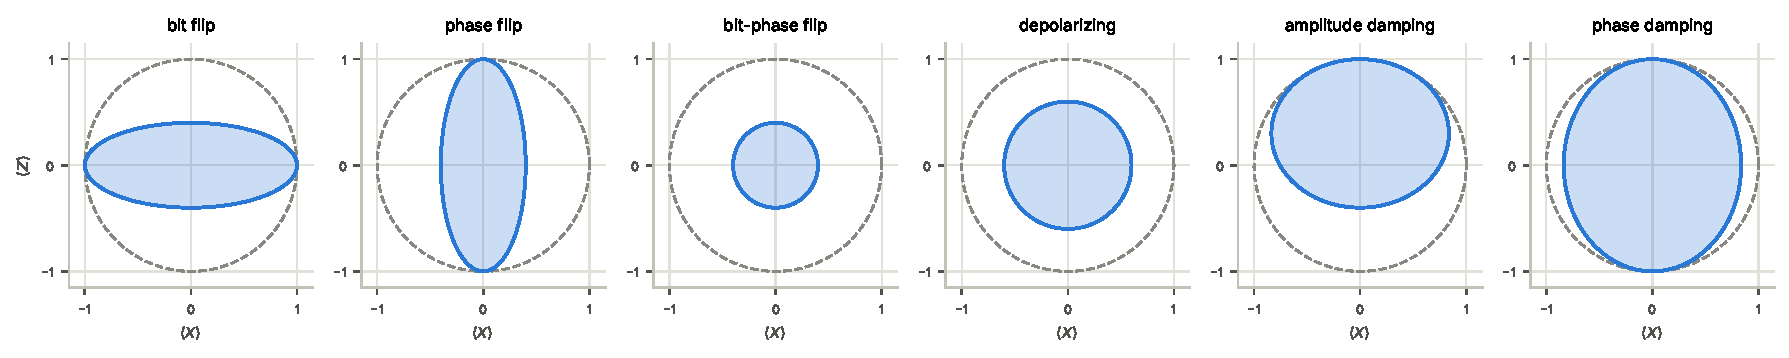
\includegraphics[width=\textwidth]{bloch_channels}\\
  \small
  $x$--$z$ cross-section of the Bloch ball (dashed) and its image (blue) for $p = \gamma = \lambda = 0.3$. Computed from the Kraus operators and checked
  with CUDA-Q density-matrix simulations (largest difference \numblochcheck).
  \begin{itemize}\itemsep0pt\scriptsize
    \item bit flip keeps $x$; phase flip keeps $z$; bit-phase flip keeps $y$ (shrinks both $x$ and $z$); depolarizing shrinks everything by $0.6$
    \item amplitude damping \key{shifts} the ball towards $\ket0$; phase damping squeezes it to the $z$-axis
  \end{itemize}
\end{frame}

\begin{frame}[label=fSingle]{Single-qubit noise models: summary}
  \footnotesize
  \begin{center}
  \renewcommand{\arraystretch}{1.25}
  \resizebox{\linewidth}{!}{%
  \begin{tabular}{lllll}
    \toprule \textbf{channel} & \textbf{Kraus operators} & \textbf{Bloch map} & \textbf{unital} & \textbf{CUDA-Q}\\ \midrule
    bit flip & $\sqrt{1-p}I$, $\sqrt pX$ & $(r_x, cr_y, cr_z)$, $c = 1 - 2p$ & yes & \texttt{BitFlipChannel}\\
    phase flip & $\sqrt{1-p}I$, $\sqrt pZ$ & $(cr_x, cr_y, r_z)$ & yes & \texttt{PhaseFlipChannel}\\
    bit-phase flip & $\sqrt{1-p}I$, $\sqrt pY$ & $(cr_x, r_y, cr_z)$ & yes & \texttt{YError}\\
    depolarizing & $\sqrt{1-p}I$, $\sqrt{p/3}\{X, Y, Z\}$ & $(1 - \frac{4p}{3})\vec r$ & yes & \texttt{DepolarizationChannel}\\
    amplitude damping & $\operatorname{diag}(1, \sqrt{1-\gamma})$, $\sqrt\gamma\ket0\!\bra1$ & $(\sqrt{1-\gamma}r_{x,y},\ \gamma + (1-\gamma)r_z)$ & no & \texttt{AmplitudeDampingChannel}\\
    phase damping & $\operatorname{diag}(1, \sqrt{1-\lambda})$, $\operatorname{diag}(0, \sqrt\lambda)$ & $(\sqrt{1-\lambda}r_{x,y},\ r_z)$ & yes & \texttt{PhaseDamping}\\
    any channel & user-defined $\{K_k\}$ & affine map & --- & \texttt{KrausChannel}\\ \bottomrule
  \end{tabular}}
  \end{center}
  \small Used by the notebook: depolarizing, bit flip, phase flip, amplitude damping (plus \texttt{Depolarization2}, \texttt{Pauli2},
  \texttt{KrausChannel} on CNOTs).
\end{frame}

% =====================================================================================
\section{Part 4: Hardware-level noise}
\begin{frame}[label=fTwoQ]{Two-qubit gate noise}
  \begin{columns}[T]
    \begin{column}{0.52\textwidth}
      \small
      Two-qubit gates are typically several times noisier than single-qubit gates (indicative). Models used by the notebook after every CNOT:
      \begin{itemize}\itemsep1pt\scriptsize
        \item depolarizing: \texttt{Depolarization2(p)} --- one joint channel, failure probability $p$
        \item bit/phase flip: \texttt{Pauli2} with $p(1-p)$ on $IX$ and $XI$ (or $IZ$, $ZI$) and $p^2$ on $XX$ ($ZZ$) = independent flips
        \item amplitude damping: \texttt{KrausChannel}$\{K_i\otimes K_j\}$ --- independent on both qubits
      \end{itemize}
      \key{No-error probability} of the 15-qubit GHZ circuit (1 H + 14 CNOT):
      depolarizing $(1-p)^{15}$; bit flip $(1-p)^{1 + 2\cdot14} = (1-p)^{29}$.
    \end{column}
    \begin{column}{0.44\textwidth}
      \begin{exampleblock}{Numbers}
        \scriptsize $p = 0.01$: depolarizing $0.99^{15} = 0.8601$; bit flip $0.99^{29} = 0.7472$.\\
        \texttt{stim}, 15-qubit GHZ at $p = 0.05$: bit flip gives population \numbfpop, parity \numbfpar.
      \end{exampleblock}
      \begin{alertblock}{Error propagation}
        \scriptsize A CNOT copies an $X$ error from control to target and a $Z$ error from target to control: errors spread through entangling layers.
      \end{alertblock}
    \end{column}
  \end{columns}
\end{frame}

\begin{frame}[label=fReadout]{Measurement errors and readout noise \tagillus}
  \begin{columns}[T]
    \begin{column}{0.46\textwidth}
      \small
      The measured \emph{bit} is wrong with some probability --- a classical error after the quantum measurement:
      \[ A = \begin{pmatrix}P(0|0) & P(0|1)\\ P(1|0) & P(1|1)\end{pmatrix},\quad \mathbf q = A\mathbf p. \]
      \scriptsize Example: $P(1|0) = 0.02$, $P(0|1) = 0.05$ (asymmetric: $\ket1$ may relax during readout). $\ket+$ is read as 1 with probability $0.485$.
      A perfect 3-qubit GHZ shows population $\frac12(0.98^3 + 0.95^3) \approx 0.899$.
    \end{column}
    \begin{column}{0.50\textwidth}
      \centering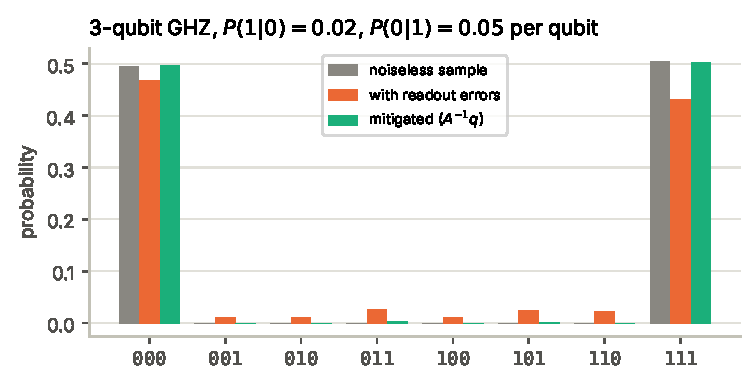
\includegraphics[width=\textwidth]{readout}\\
      {\scriptsize Noiseless CUDA-Q sample, readout errors applied per bit: population \numropopideal{} $\to$ \numropopnoisy; mitigated \numropopmit.}
    \end{column}
  \end{columns}
  \small \hl{Not modelled in \texttt{Noise\_Simulation.ipynb}}: its measurements are ideal.
\end{frame}

\begin{frame}[label=fT1T2]{Thermal relaxation: $T_1$ and $T_2$}
  \begin{columns}[T]
    \begin{column}{0.52\textwidth}
      \small
      \begin{itemize}\itemsep2pt
        \item $T_1$ (relaxation): $\rho_{11}(t) = \rho_{11}(0)e^{-t/T_1}$; per step $\gamma = 1 - e^{-\Delta t/T_1}$
        \item $T_2$ (coherence): $|\rho_{01}(t)| = |\rho_{01}(0)|e^{-t/T_2}$
        \item $\frac{1}{T_2} = \frac{1}{2T_1} + \frac{1}{T_\varphi}$, hence $T_2 \le 2T_1$
        \item at finite temperature the qubit relaxes to a thermal state, not exactly to $\ket0$ (generalized amplitude damping)
      \end{itemize}
      \begin{exampleblock}{Worked examples}
        \scriptsize $T_1 = 50\,\mu$s: $P(1) = \frac12$ after $T_1\ln2 = 34.7\,\mu$s.\\
        $T_1 = 100$, $T_\varphi = 200\,\mu$s $\Rightarrow T_2 = 100\,\mu$s.\\
        $T_2 = 100\,\mu$s, 50 ns gates: $e^{-nt_g/T_2} \ge 0.9$ for $n \le 210$ gates.
      \end{exampleblock}
    \end{column}
    \begin{column}{0.44\textwidth}
      \begin{block}{Typical orders of magnitude}
        \scriptsize superconducting qubits: $T_1, T_2 \sim 10$--$500\,\mu$s, gates $20$--$500$ ns; trapped ions: $T_2$ seconds or more, gates $\mu$s--ms.
        Ratios coherence/gate time matter, not absolute times. (Indicative literature values, not measured here.)
      \end{block}
    \end{column}
  \end{columns}
\end{frame}

\begin{frame}[label=fT1T2fig]{$T_1$ and $T_2$ simulated step by step \tagillus}
  \begin{columns}[T]
    \begin{column}{0.56\textwidth}
      \centering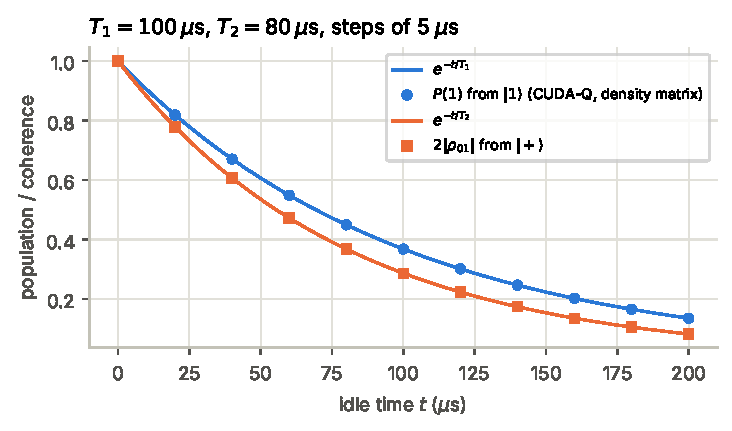
\includegraphics[width=\textwidth]{t1t2}
    \end{column}
    \begin{column}{0.40\textwidth}
      \small
      Each 5\,$\mu$s idle step applies one \texttt{KrausChannel} = amplitude damping $\gamma$ followed by phase damping $\lambda$, with
      $T_\varphi = \numtphi\,\mu$s chosen so that $T_2 = 80\,\mu$s.
      \begin{itemize}\itemsep1pt\scriptsize
        \item CUDA-Q density matrix agrees with $e^{-t/T_1}$, $e^{-t/T_2}$ to \numtonecheck
        \item the identity ``idle'' gate is \texttt{rx(idle)} with \texttt{idle = 0.0} passed at run time (see ``Pitfalls'')
      \end{itemize}
    \end{column}
  \end{columns}
\end{frame}

\begin{frame}[label=fRates]{Error rates, gate errors and benchmarking}
  \begin{columns}[T]
    \begin{column}{0.52\textwidth}
      \small
      \begin{itemize}\itemsep2pt
        \item \key{process fidelity} $F_{\text{pro}} = \braket{\Phi^+|J(\E)|\Phi^+}$ --- depolarizing: $1 - p$
        \item \key{average gate fidelity} $F_{\text{avg}} = \frac{dF_{\text{pro}} + 1}{d+1}$ --- depolarizing qubit: $1 - \frac{2p}{3}$
        \item \key{error rate} $r = 1 - F_{\text{avg}}$; $p = 0.003 \Rightarrow r = 0.002$
        \item \key{randomized benchmarking}: random Clifford sequences of length $m$; survival $A\alpha^m + B$; $r = \frac{(d-1)(1-\alpha)}{d}$
          ($\alpha = 0.99 \Rightarrow r = 0.005$); robust to SPAM errors
      \end{itemize}
    \end{column}
    \begin{column}{0.44\textwidth}
      \begin{alertblock}{Average $\neq$ worst case}
        \scriptsize A coherent over-rotation and a stochastic error with the same $r$ give very different results after many gates (Part 1). RB reports the
        average under twirling.
      \end{alertblock}
      \begin{block}{In this repository}
        \scriptsize RB and process tomography are \tagtheory; the notebook characterises circuits by population, parity, Hellinger and state fidelity.
      \end{block}
    \end{column}
  \end{columns}
\end{frame}

% =====================================================================================
\section{Part 5: Simulating noise with CUDA-Q}
\begin{frame}[label=fExec]{Noise channels in circuit execution}
  \begin{columns}[T]
    \begin{column}{0.52\textwidth}
      \small
      A noisy circuit = ideal gates, each followed by its channel:
      \[ \rho_{\text{out}} = \E_G\circ\,\mathcal U_G\circ\cdots\circ\E_1\circ\,\mathcal U_1(\rho_0),\quad \mathcal U(\rho) = U\rho U^\dagger. \]
      \key{Accumulation}: for Pauli channels with error probability $p$ at $G$ locations, the error-free branch has weight $(1-p)^G$, so
      \[ F \ge (1-p)^G \approx e^{-pG}. \]
      Deeper and wider circuits tolerate proportionally less noise.
    \end{column}
    \begin{column}{0.44\textwidth}
      \begin{center}
      \begin{quantikz}[row sep=0.2cm, column sep=0.22cm]
        \lstick{$\ket0$} & \gate{H} & \gate[style={fill=qorange!15}]{\E} & \ctrl{1} & \gate[2,style={fill=qorange!15}]{\E_2} & \meter{}\\
        \lstick{$\ket0$} & \qw & \qw & \targ{} & & \meter{}
      \end{quantikz}
      \end{center}
      \begin{exampleblock}{The bound is not tight}
        \scriptsize 6-qubit GHZ, depolarizing $p = 0.01$: $F = \numdmfid > 0.99^6 = 0.9415$ --- e.g.\ $Z\otimes Z$ after a CNOT leaves GHZ unchanged.
        For non-Pauli noise (amplitude damping) the notebook does not claim the bound.
      \end{exampleblock}
    \end{column}
  \end{columns}
\end{frame}

\begin{frame}[fragile,label=fInject]{Noise injection in CUDA-Q \tagimpl}
  \begin{columns}[T]
    \begin{column}{0.55\textwidth}
\begin{lstlisting}
model = cudaq.NoiseModel()
model.add_all_qubit_channel("h",
        cudaq.DepolarizationChannel(p))
model.add_all_qubit_channel("x",
        cudaq.Depolarization2(p), num_controls=1)

# shot-based (stim, trajectories)
counts = cudaq.sample(ghz_z, 15, shots_count=10000,
                      noise_model=model)
# exact expectation value (density matrix)
cudaq.set_target("density-matrix-cpu")
zz = cudaq.observe(kernel, cudaq.spin.z(0),
                   noise_model=model).expectation()
\end{lstlisting}
    \end{column}
    \begin{column}{0.42\textwidth}
      \scriptsize
      \begin{itemize}\itemsep1pt
        \item a \texttt{NoiseModel} attaches channels to \emph{gate names}; \texttt{num\_controls=1} selects CNOTs
        \item the channel acts \emph{after} every matching gate, on the qubits it touches
        \item \texttt{sample} / \texttt{observe} take \texttt{noise\_model=}; \texttt{get\_state} does not (CUDA-Q 0.16) $\Rightarrow$
          \texttt{cudaq.set\_noise(model)} \dots\ \texttt{unset\_noise()}
        \item only noise-capable targets apply it: \texttt{stim}, \texttt{density-matrix-cpu}, \texttt{nvidia} (trajectories)
      \end{itemize}
    \end{column}
  \end{columns}
\end{frame}

\begin{frame}[fragile,label=fPitfalls]{Pitfalls found while preparing these slides \tagillus}
  \begin{columns}[T]
    \begin{column}{0.5\textwidth}
      \begin{alertblock}{1. Constant identity gates vanish}
        \scriptsize
\begin{lstlisting}[basicstyle=\ttfamily\tiny]
rx(0.0, q[0])   # constant: removed -> no noise
rx(idle, q[0])  # idle = 0.0 passed at run time
\end{lstlisting}
        With \texttt{DepolarizationChannel(0.3)} on \texttt{rx}: $\langle Z\rangle = 1.0$ vs.\ $0.6$. Idle noise needs a gate that survives compilation.
      \end{alertblock}
    \end{column}
    \begin{column}{0.46\textwidth}
      \begin{alertblock}{2. Keep the noise model alive}
        \scriptsize \texttt{cudaq.set\_noise(build\_noise\_model(...))} with a temporary object crashed the process (segmentation fault) in
        \texttt{get\_state}: the model was garbage-collected. The notebook keeps a reference --- its comment says so.
      \end{alertblock}
      \begin{alertblock}{3. Noiseless targets ignore noise}
        \scriptsize \texttt{qpp-cpu} / \texttt{nvidia} without a noise-capable method return ideal results; the notebook refuses \texttt{statevector}.
      \end{alertblock}
    \end{column}
  \end{columns}
\end{frame}

\begin{frame}[label=fMethods]{Three ways to simulate noise}
  \footnotesize
  \begin{center}
  \resizebox{\linewidth}{!}{%
  \begin{tabular}{lllll}
    \toprule \textbf{method} & \textbf{CUDA-Q target} & \textbf{memory} & \textbf{supports} & \textbf{result}\\ \midrule
    density matrix & \texttt{density-matrix-cpu} & $16\cdot4^N$ B ($N = 13$: 1.07 GB) & any Kraus channel, any gate & exact $\rho$\\
    trajectories (Monte Carlo) & \texttt{nvidia} + noise model (GPU) & $16\cdot2^N$ B per trajectory & any channel & statistical\\
    stabilizer & \texttt{stim} & $\sim N^2$ bits & Clifford gates + Pauli noise only & statistical, hundreds of qubits\\ \bottomrule
  \end{tabular}}
  \end{center}
  \begin{columns}[T]
    \begin{column}{0.5\textwidth}
      \scriptsize
      \key{Trajectories}: for each shot, pick Kraus jumps at random (probability $\operatorname{Tr}K\rho K^\dagger$), keep a pure state; the average over many
      trajectories reproduces $\rho$. Memory ratio to the density matrix at $N = 20$: $2^{20} \approx 10^6$.
    \end{column}
    \begin{column}{0.46\textwidth}
      \scriptsize
      \key{Stabilizer}: Gottesman--Knill; GHZ with depolarizing noise is fine, rotations by arbitrary angles, $T$ gates or amplitude damping are not.
      The notebook raises an error instead of silently ignoring such noise.
    \end{column}
  \end{columns}
\end{frame}

\begin{frame}[label=fShots]{Shot-based simulation}
  \begin{columns}[T]
    \begin{column}{0.52\textwidth}
      \small
      \begin{itemize}\itemsep2pt
        \item \texttt{stim} / trajectories: every shot samples one error pattern and one outcome $\Rightarrow$ counts directly
        \item density matrix: probabilities $= \operatorname{diag}\rho$ exactly; the notebook draws \texttt{SHOTS} counts with a seeded
          \texttt{multinomial} (statistically identical to measuring)
        \item why? noisy \texttt{cudaq.sample} on \texttt{density-matrix-cpu} took $\approx 115$ s at 10 qubits (README) vs.\ $\approx1$ s for \texttt{get\_state}
        \item shot noise: $\pm\sqrt{P(1-P)/S}$; at $S = 10^4$ and $P = 0.9$: $\pm0.003$
      \end{itemize}
    \end{column}
    \begin{column}{0.44\textwidth}
      \begin{exampleblock}{Counts $\to$ figures of merit}
        \scriptsize $X$-basis counts \texttt{\{00:450, 11:400, 01:80, 10:70\}}: parity $= (850 - 150)/1000 = 0.70$.\\[2pt]
        Ideal $P = (0.5, 0, 0, 0.5)$, noisy $Q = (0.45, 0.05, 0.05, 0.45)$: Hellinger $F_H = 0.90$, TVD $= 0.10$.
      \end{exampleblock}
    \end{column}
  \end{columns}
\end{frame}

\begin{frame}[label=fNoisyVs]{Noisy versus noiseless execution: what to measure}
  \footnotesize
  \begin{center}
  \resizebox{\linewidth}{!}{%
  \begin{tabular}{llll}
    \toprule \textbf{figure of merit} & \textbf{definition} & \textbf{sensitive to} & \textbf{needs}\\ \midrule
    GHZ population & $P(0\cdots0) + P(1\cdots1)$ & bit flips & $Z$-basis counts\\
    parity & $\langle X^{\otimes N}\rangle = P(\text{even}) - P(\text{odd})$ ($X$ basis) & phase flips (and bit flips) & extra run with Hadamards\\
    Hellinger fidelity & $(\sum_x\sqrt{p_xq_x})^2$ & any change of the distribution & counts\\
    total variation distance & $\frac12\sum_x|p_x - q_x|$ & any change & counts\\
    state fidelity & $\braket{\psi|\rho|\psi}$ & everything, incl.\ coherences & density matrix\\
    purity & $\operatorname{Tr}\rho^2$ & mixedness & density matrix\\
    no-error probability & $(1-p)^G$ & --- (a bound, for Pauli noise) & gate count\\ \bottomrule
  \end{tabular}}
  \end{center}
  \small All are computed in \texttt{Noise\_Simulation.ipynb} \tagimpl; the noiseless run ($p = 0$) is always included as a check.
\end{frame}

\begin{frame}[label=fStruct]{The structure of \texttt{Noise\_Simulation.ipynb} \tagimpl}
  \begin{columns}[T]
    \begin{column}{0.48\textwidth}
      \scriptsize
      \begin{tabular}{rl}
        \toprule \textbf{Sec.} & \textbf{Content}\\ \midrule
        1 & problem statement, channels, figures of merit\\
        2 & imports, versions, GPUs\\
        3 & \key{input parameters} (only cell to edit)\\
        4 & validation, gate counts, \texttt{build\_noise\_model}\\
        5 & utilities, \texttt{auto} method choice, backend\\
        6 & expected results, memory, time estimate\\
        7 & kernels, drawing, circuit statistics\\
        8 & execution with memory monitoring\\
        9 & ideal vs.\ noisy plots and sweep table\\
        10 & final benchmark report (JSON + PNG)\\ \bottomrule
      \end{tabular}
    \end{column}
    \begin{column}{0.48\textwidth}
      \scriptsize
      \textbf{Section 3 defaults}\\
      \texttt{N\_QUBITS = 15}, \texttt{CIRCUIT = "ghz"} (or \texttt{"mirror"}, \texttt{MIRROR\_LAYERS = 2})\\
      \texttt{NOISE\_MODEL = "depolarizing"} (\texttt{bit\_flip}, \texttt{phase\_flip}, \texttt{amplitude\_damping})\\
      \texttt{NOISE\_PROBABILITY = 0.01}\\
      \texttt{NOISE\_SWEEP = [0, 0.001, 0.002, 0.005, 0.01, 0.02, 0.05, 0.1]}\\
      \texttt{MEASURE\_X\_BASIS = True}, \texttt{SHOTS = 10000}, \texttt{SEED = 42}\\
      \texttt{BACKEND = "auto"}, \texttt{SIMULATION\_METHOD = "auto"}\\[3pt]
      Exports (\texttt{exports/noise/}, not committed): circuit drawing (\texttt{.txt}, \texttt{.png}), QIR (\texttt{.ll}), report (\texttt{.json}, \texttt{.png}).
    \end{column}
  \end{columns}
\end{frame}

\begin{frame}[fragile,label=fModel]{\texttt{build\_noise\_model}, line by line}
  \begin{columns}[T]
    \begin{column}{0.58\textwidth}
\begin{lstlisting}[basicstyle=\ttfamily\tiny]
def build_noise_model(kind, p):
    model = cudaq.NoiseModel()
    if p == 0.0:
        return model                     # empty = noiseless
    if kind == "depolarizing":
        one, two = cudaq.DepolarizationChannel(p), cudaq.Depolarization2(p)
    elif kind == "bit_flip":
        probs = [0.0] * 15               # Pauli2 order: IX IY IZ XI XX ...
        probs[0] = probs[3] = p * (1 - p)    # flip on one qubit only
        probs[4] = p * p                     # flip on both qubits
        one, two = cudaq.BitFlipChannel(p), cudaq.Pauli2(probs)
    elif kind == "phase_flip":
        probs = [0.0] * 15
        probs[2] = probs[11] = p * (1 - p)   # IZ and ZI
        probs[14] = p * p                    # ZZ
        one, two = cudaq.PhaseFlipChannel(p), cudaq.Pauli2(probs)
    else:                                # amplitude damping
        k0 = np.array([[1, 0], [0, np.sqrt(1 - p)]], dtype=complex)
        k1 = np.array([[0, np.sqrt(p)], [0, 0]], dtype=complex)
        one = cudaq.AmplitudeDampingChannel(p)
        two = cudaq.KrausChannel([np.kron(a, b) for a in (k0, k1)
                                               for b in (k0, k1)])
    for gate in ("h", "x", "ry", "rz"):
        model.add_all_qubit_channel(gate, one)
    model.add_all_qubit_channel("x", two, num_controls=1)
    return model
\end{lstlisting}
    \end{column}
    \begin{column}{0.39\textwidth}
      \scriptsize
      \begin{itemize}\itemsep1pt
        \item $p = 0$: an empty model, the noiseless reference
        \item \texttt{Pauli2} with $p(1-p), p(1-p), p^2$: exactly two independent single-qubit flips
        \item amplitude damping on CNOTs: the 4 products $K_i\otimes K_j$ --- a valid two-qubit Kraus set
        \item same $p$ for every gate; no idle noise, no measurement noise, no crosstalk
        \item checked in the verifier: CUDA-Q's channels equal the Kraus sets of the slides
      \end{itemize}
    \end{column}
  \end{columns}
\end{frame}

\begin{frame}[fragile,label=fKernels]{Kernels and execution, line by line}
  \begin{columns}[T]
    \begin{column}{0.55\textwidth}
\begin{lstlisting}[basicstyle=\ttfamily\tiny]
@cudaq.kernel
def ghz_x(n: int):
    qubits = cudaq.qvector(n)
    h(qubits[0])
    for i in range(n - 1):
        x.ctrl(qubits[i], qubits[i + 1])
    h(qubits)                     # X-basis readout
    mz(qubits)

def run_once(kernels, kind, p, basis):
    model = build_noise_model(kind, p)
    if chosen_method == "density_matrix":
        cudaq.set_noise(model)
        try:
            rho = np.array(cudaq.get_state(kernels[name], *args))
        finally:
            cudaq.unset_noise()
        counts, exact = as_counts_from_rho(rho, N_QUBITS, SHOTS)
        return counts, exact, rho
    result = cudaq.sample(kernels[name], *args,
                          shots_count=SHOTS, noise_model=model)
    return {b: c for b, c in result.items()}, None, None
\end{lstlisting}
    \end{column}
    \begin{column}{0.42\textwidth}
      \scriptsize
      \begin{itemize}\itemsep1pt
        \item GHZ in the $Z$ basis (\texttt{ghz\_z}) and the $X$ basis (\texttt{ghz\_x}: extra Hadamards, also noisy)
        \item mirror circuit: $R_Y R_Z$ layers + CNOT ladder, then the inverse --- ideally $\ket{0\cdots0}$, non-Clifford
        \item the noise model is \emph{not} drawn: channels are inserted at simulation time
        \item \texttt{try/finally}: the global noise is always removed again
        \item every $p$ of the sweep runs in both bases ($8 \times 2 = 16$ runs)
      \end{itemize}
    \end{column}
  \end{columns}
\end{frame}

\begin{frame}[label=fAuto]{Method selection and safeguards \tagimpl}
  \begin{columns}[T]
    \begin{column}{0.5\textwidth}
      \small \texttt{SIMULATION\_METHOD = "auto"}:
      \begin{enumerate}\itemsep1pt\scriptsize
        \item a GPU is visible $\to$ \texttt{trajectory} (\texttt{nvidia})
        \item CPU, GHZ, Pauli noise $\to$ \texttt{stabilizer} (\texttt{stim})
        \item otherwise $\to$ \texttt{density\_matrix} (\texttt{density-matrix-cpu})
      \end{enumerate}
      \scriptsize Example: CPU, GHZ, amplitude damping $\Rightarrow$ density matrix.
    \end{column}
    \begin{column}{0.46\textwidth}
      \begin{alertblock}{Refused on purpose}
        \scriptsize
        \begin{itemize}\itemsep1pt
          \item \texttt{stabilizer} with amplitude damping or the mirror circuit
          \item \texttt{statevector} (ignores noise)
          \item \texttt{BACKEND = "hardware"}: ``noise models are a simulator feature''
          \item density matrix on GPU, trajectories on CPU (not offered by CUDA-Q)
        \end{itemize}
      \end{alertblock}
    \end{column}
  \end{columns}
\end{frame}

\begin{frame}[label=fGlance]{The implementation at a glance}
  \scriptsize
  \begin{center}
  \resizebox{\linewidth}{!}{%
  \begin{tabular}{ll@{\hspace{1.5em}}ll}
    \toprule
    simulator (recorded) & \texttt{stim} (CPU), CUDA-Q 0.16.0 & shots & 10\,000, seed 42\\
    other methods & \texttt{density-matrix-cpu}, \texttt{nvidia} trajectories (GPU, not run) & circuits & GHZ (default), mirror\\
    qubits & 15 (density matrix: keep $\le 10$; \texttt{stim}: hundreds) & gate locations & 1 H + 14 CNOT (GHZ)\\
    noise models & depolarizing, bit flip, phase flip, amplitude damping & error probability & $p$ per gate, sweep $0 \dots 0.1$\\
    gate-level noise & after \texttt{h, x, ry, rz} and every CNOT & measurement noise & none\\
    fidelity measures & population, parity, Hellinger, TVD, state fidelity, purity & bound & $(1-p)^G$ (Pauli noise)\\
    benchmark output & time phases, memory timeline, JSON report & hardware & refused (simulator only)\\ \bottomrule
  \end{tabular}}
  \end{center}
\end{frame}

\begin{frame}[label=fRec]{Recorded versus re-executed results}
  \begin{columns}[T]
    \begin{column}{0.5\textwidth}
      \centering\footnotesize
      \resizebox{\linewidth}{!}{% GENERATED by make_figures.py - do not edit
\begin{tabular}{rcccr}\toprule
$p$ & population & $\langle X^{\otimes15}\rangle$ & $(1-p)^G$ & outcomes \\ \midrule
0 & 1.0000 & 1.0000 & 1.0000 & 2 \\
0.001 & 0.9873 & 0.9660 & 0.9851 & 48 \\
0.002 & 0.9807 & 0.9324 & 0.9704 & 56 \\
0.005 & 0.9458 & 0.8374 & 0.9276 & 64 \\
0.01 & 0.8936 & 0.6910 & 0.8601 & 96 \\
0.02 & 0.8009 & 0.4834 & 0.7386 & 196 \\
0.05 & 0.5724 & 0.1518 & 0.4633 & 564 \\
0.1 & 0.3232 & 0.0160 & 0.2059 & 1165 \\
\bottomrule
\end{tabular}
}\\[2pt]
      {\scriptsize Re-executed with the notebook's model, seed and call order on \texttt{stim}: \numreproduced.}
    \end{column}
    \begin{column}{0.46\textwidth}
      \small
      \begin{itemize}\itemsep1pt\scriptsize
        \item population $\ge (1-p)^G$ everywhere: the bound holds and is not tight
        \item the parity falls much faster: phase errors and the extra Hadamards
        \item outcomes: 2 $\to$ 1165 --- probability leaks into many bitstrings
        \item recorded run time 0.25 s (16 runs); re-executed sweep \numstimtime{} s
        \item the density-matrix path is not part of the recorded outputs; it was run for these slides (next slides)
      \end{itemize}
    \end{column}
  \end{columns}
\end{frame}

\begin{frame}[label=fKinds]{Bit flips, phase flips and depolarizing noise compared \tagillus}
  \begin{columns}[T]
    \begin{column}{0.48\textwidth}
      \centering\footnotesize
      % GENERATED by make_figures.py - do not edit
\begin{tabular}{lccc}\toprule
noise & $p$ & Z population & X parity \\ \midrule
depolarizing & 0.01 & 0.8936 & 0.6920 \\
depolarizing & 0.05 & 0.5728 & 0.1522 \\
bit flip & 0.01 & 0.7501 & 0.7382 \\
bit flip & 0.05 & 0.2319 & 0.1996 \\
phase flip & 0.01 & 1.0000 & 0.5580 \\
phase flip & 0.05 & 1.0000 & 0.0504 \\
\bottomrule
\end{tabular}
\\[2pt]
      {\scriptsize 15-qubit GHZ, notebook model, \texttt{stim}, 10\,000 shots.}
    \end{column}
    \begin{column}{0.48\textwidth}
      \small
      \begin{itemize}\itemsep1pt\scriptsize
        \item phase flips: population exactly 1, parity collapses --- invisible in the $Z$ basis
        \item bit flips: both drop; two failure chances per CNOT make them harsher than depolarizing at the same $p$
        \item depolarizing: $\frac23$ of single-qubit errors flip $Z$ outcomes, $\frac23$ flip phases
        \item the README's ``parity 0.56'' for phase flips is reproduced (0.5580 at $p = 0.01$)
      \end{itemize}
    \end{column}
  \end{columns}
\end{frame}

\begin{frame}[label=fDMres]{The density-matrix path: fidelity and purity \tagillus}
  \begin{columns}[T]
    \begin{column}{0.56\textwidth}
      \centering\footnotesize
      \resizebox{\linewidth}{!}{% GENERATED by make_figures.py - do not edit
\begin{tabular}{lcccc}\toprule
noise & $p$ & $F = \langle\mathrm{GHZ}|\rho|\mathrm{GHZ}\rangle$ & $\mathrm{Tr}\,\rho^2$ & population \\ \midrule
depolarizing & 0.01 & 0.9492 & 0.9013 & 0.9633 \\
depolarizing & 0.05 & 0.7686 & 0.5959 & 0.8275 \\
bit flip & 0.01 & 0.9045 & 0.8191 & 0.9045 \\
bit flip & 0.05 & 0.6009 & 0.3749 & 0.6009 \\
phase flip & 0.01 & 0.9004 & 0.8206 & 1.0000 \\
phase flip & 0.05 & 0.6569 & 0.5492 & 1.0000 \\
amplitude damping & 0.01 & 0.9495 & 0.9034 & 0.9527 \\
amplitude damping & 0.05 & 0.7824 & 0.6453 & 0.8106 \\
\bottomrule
\end{tabular}
}\\[2pt]
      {\scriptsize 6-qubit GHZ, notebook model, \texttt{set\_noise} + \texttt{get\_state}. Independent NumPy simulation agrees to \numdmcross.}
    \end{column}
    \begin{column}{0.40\textwidth}
      \small
      \begin{itemize}\itemsep1pt\scriptsize
        \item state fidelity and purity need $\rho$: only this path gives them
        \item phase flip: population 1 but fidelity $0.66$ at $p = 0.05$
        \item bit flip: fidelity $=$ population ($X$-type errors never create a relative phase between $\ket{0\cdots0}$ and $\ket{1\cdots1}$)
        \item amplitude damping: outcomes biased towards $0\cdots0$
        \item mirror circuit (4 qubits, \nummirrorgates{} noisy gates, $p = 0.01$): success \nummirrorone{} $\ge$ bound \nummirrorlb; noiseless \nummirrorzero
      \end{itemize}
    \end{column}
  \end{columns}
\end{frame}

\begin{frame}[label=fAlgs]{Noise on QFT, QAOA and VQE circuits \tagillus}
  \begin{columns}[T]
    \begin{column}{0.5\textwidth}
      \centering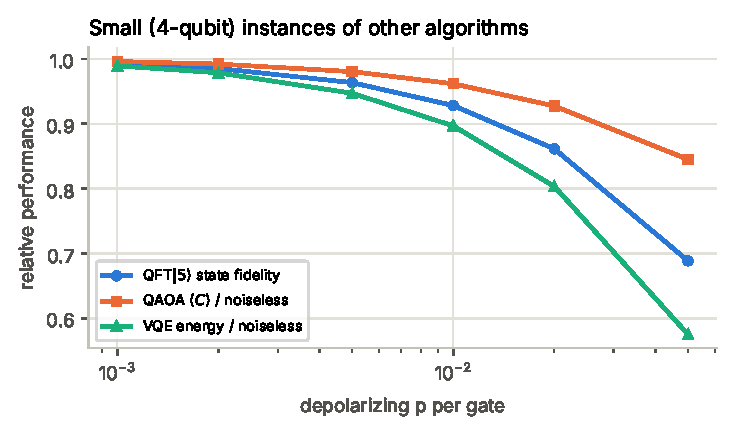
\includegraphics[width=0.92\textwidth]{algorithms}\\[2pt]
      \resizebox{\linewidth}{!}{% GENERATED by make_figures.py - do not edit
\begin{tabular}{rccc}\toprule
$p$ & QFT state fidelity & QAOA $\langle C\rangle$ (ring, 4) & VQE energy (TFIM, 4) \\ \midrule
0 & 1.0000 & 3.0000 & -3.4141 \\
0.001 & 0.9926 & 2.9879 & -3.3772 \\
0.002 & 0.9852 & 2.9759 & -3.3406 \\
0.005 & 0.9634 & 2.9408 & -3.2332 \\
0.01 & 0.9280 & 2.8849 & -3.0612 \\
0.02 & 0.8613 & 2.7819 & -2.7427 \\
0.05 & 0.6887 & 2.5350 & -1.9638 \\
\bottomrule
\end{tabular}
}
    \end{column}
    \begin{column}{0.46\textwidth}
      \scriptsize
      Small 4-qubit versions on \texttt{density-matrix-cpu}, depolarizing $p$ after every gate:
      \begin{itemize}\itemsep1pt
        \item \key{QFT} of $\ket{5}$ (H and controlled phases): state fidelity \numqftone{} at $p = 0.01$
        \item \key{QAOA}, ring of 4, $p = 1$, angles optimised without noise: $\langle C\rangle$ $\numqaoacut \to \numqaoaone$
        \item \key{VQE}, 4-qubit TFIM, hardware-efficient ansatz (exact ground energy \numvqeexact, noiseless VQE \numvqeideal): $\numvqeone$
      \end{itemize}
      These are \emph{not} the circuits of \texttt{QFT.ipynb}, \texttt{QAOA.ipynb}, \texttt{VQE.ipynb} (those notebooks model only shot noise).
      Noisy VQE energies stay above the ground energy (the variational bound still holds for mixed states) but move away from it.
    \end{column}
  \end{columns}
\end{frame}

\begin{frame}[label=fScale]{Noise benchmarking: the cost of simulation \tagillus}
  \begin{columns}[T]
    \begin{column}{0.56\textwidth}
      \centering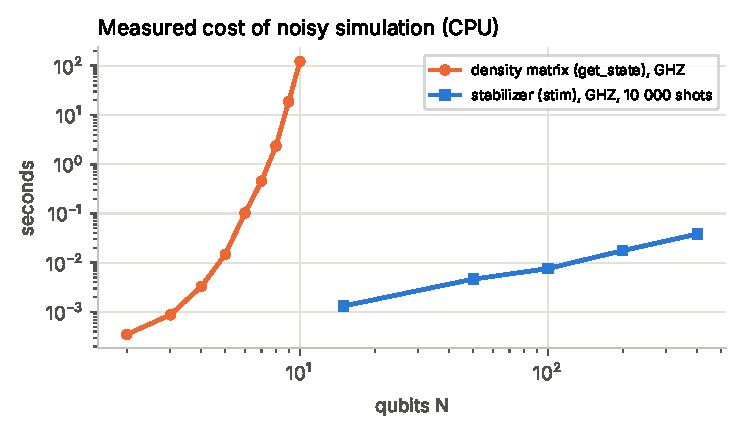
\includegraphics[width=\textwidth]{scaling}
    \end{column}
    \begin{column}{0.40\textwidth}
      \small
      Measured on the 4-core CPU container:
      \begin{itemize}\itemsep1pt\scriptsize
        \item density matrix, GHZ with depolarizing noise: 10 qubits took \numdmten{} s for one \texttt{get\_state} --- growing about $\times7$ per qubit
        \item \texttt{stim}: 400 qubits, 10\,000 shots in \numstimfourhundred{} s
        \item GPU trajectories would sit in between (not measured)
      \end{itemize}
      \scriptsize Benchmark noise studies with the cheapest exact method for the circuit class.
    \end{column}
  \end{columns}
\end{frame}

% =====================================================================================
\section{Part 6: Mitigation, correction and hardware}
\begin{frame}[label=fMitig]{Error mitigation, correction and simulation are different things}
  \footnotesize
  \begin{center}
  \resizebox{\linewidth}{!}{%
  \begin{tabular}{llll}
    \toprule & \textbf{noise simulation} & \textbf{error mitigation} & \textbf{error correction}\\ \midrule
    goal & \emph{predict} what noisy hardware does & \emph{estimate} ideal expectation values from noisy runs & \emph{protect} the quantum state\\
    acts on & a classical model & measurement statistics (post-processing) & the state, during the computation\\
    examples & density matrix, trajectories, stim & ZNE, readout mitigation, PEC, symmetry checks & repetition code, surface code\\
    cost & classical memory/time & extra shots (variance grows) & many qubits, fast feedback, below threshold\\
    in this repository & \texttt{Noise\_Simulation.ipynb} \tagimpl & lecture experiments \tagillus & lecture experiment \tagillus\\ \bottomrule
  \end{tabular}}
  \end{center}
  \small Dynamical decoupling is different again: it changes the physical evolution during idle periods.
\end{frame}

\begin{frame}[label=fZNE]{Zero-noise extrapolation (ZNE)}
  \begin{columns}[T]
    \begin{column}{0.52\textwidth}
      \small
      Measure $E(\lambda)$ at amplified noise $\lambda \ge 1$ and extrapolate to $\lambda = 0$.
      \begin{itemize}\itemsep1pt
        \item linear: $E_0 = 2E(1) - E(2)$
        \item Richardson ($\lambda = 1, 2, 3$): $E_0 = 3E(1) - 3E(2) + E(3)$
        \item exponential: $E = ae^{-b\lambda}$
      \end{itemize}
      \key{Amplifying noise on hardware}: gate folding $G \to GG^\dagger G$ ($\lambda = 3$ for that gate; fold 4 of 10 gates: $\lambda = 1.8$), or pulse stretching.
    \end{column}
    \begin{column}{0.44\textwidth}
      \begin{alertblock}{Costs and caveats}
        \scriptsize
        \begin{itemize}\itemsep1pt
          \item biased: depends on the model ($0.80, 0.64 \to$ linear $0.96$, exponential $1.00$)
          \item variance amplified by $\sqrt{\sum\gamma_k^2}$ ($\sqrt{19} \approx 4.4$ for Richardson)
          \item only expectation values, not states; no protection of long computations
        \end{itemize}
      \end{alertblock}
    \end{column}
  \end{columns}
\end{frame}

\begin{frame}[label=fZNEfig]{ZNE on a GHZ parity \tagillus}
  \begin{columns}[T]
    \begin{column}{0.5\textwidth}
      \centering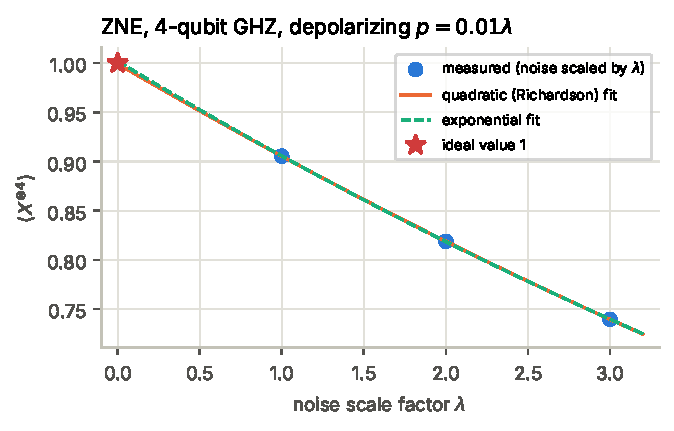
\includegraphics[width=\textwidth]{zne}
    \end{column}
    \begin{column}{0.46\textwidth}
      \small
      4-qubit GHZ, $\langle X^{\otimes4}\rangle$, notebook depolarizing model at $p = 0.01\lambda$ (exact density matrix):
      \begin{center}\scriptsize
      \begin{tabular}{lccc}\toprule $\lambda$ & 1 & 2 & 3\\ \midrule value & \numzneone & \numznetwo & \numznethree\\ \bottomrule\end{tabular}
      \end{center}
      \scriptsize linear \numznelin, Richardson \numznequad, exponential \numzneexp{} ($> 1$: unphysical overshoot).
      Here $p$ is scaled in software; on hardware the noise must be amplified physically.
    \end{column}
  \end{columns}
\end{frame}

\begin{frame}[label=fROM]{Readout-error mitigation \tagillus}
  \begin{columns}[T]
    \begin{column}{0.52\textwidth}
      \small
      \begin{enumerate}\itemsep1pt
        \item calibrate: prepare each basis state, measure, estimate $A$ (columns = prepared states)
        \item measure the experiment: frequencies $\mathbf q$
        \item solve $A\mathbf p = \mathbf q$ (least squares with $\mathbf p \ge 0$ in practice)
      \end{enumerate}
      \begin{exampleblock}{Worked example}
        \scriptsize $P(0|0) = 0.98$, $P(0|1) = 0.05$, measured $q_0 = 0.60$: $0.93p_0 = 0.55 \Rightarrow p_0 = 0.591$.
      \end{exampleblock}
    \end{column}
    \begin{column}{0.44\textwidth}
      \small 3-qubit GHZ (figure on the readout slide): population \numropopnoisy{} $\to$ \numropopmit.
      \begin{alertblock}{Limits}
        \scriptsize negative quasi-probabilities (minimum here \numrominneg); shot noise amplified; $2^N\times2^N$ matrix $\Rightarrow$ tensor-product or
        correlated sparse models for many qubits; does nothing for gate errors.
      \end{alertblock}
    \end{column}
  \end{columns}
\end{frame}

\begin{frame}[label=fDD]{Dynamical decoupling}
  \begin{columns}[T]
    \begin{column}{0.52\textwidth}
      \small
      An idle qubit with an unknown but \emph{static} detuning $\delta$ acquires the phase $\delta t$. A $\pi$ pulse in the middle reverses the sign of the
      phase accumulated afterwards (Hahn echo):
      \[ R_Z(\tfrac\varphi2)\,X\,R_Z(\tfrac\varphi2) = X\quad (XR_Z(a)X = R_Z(-a)). \]
      \begin{center}
      \begin{quantikz}[row sep=0.2cm, column sep=0.3cm]
        \lstick{$\ket+$} & \gate{\text{idle } t/2} & \gate{X} & \gate{\text{idle } t/2} & \gate{X} & \meter{}
      \end{quantikz}
      \end{center}
      Sequences (CPMG, XY4, \dots) repeat this to suppress noise slower than the pulse spacing.
    \end{column}
    \begin{column}{0.44\textwidth}
      \begin{exampleblock}{Quasi-static detuning, $\sigma = 1$ rad/$\mu$s}
        \scriptsize Free: $\overline{\langle X\rangle} = e^{-\sigma^2t^2/2}$, at $t = 2\,\mu$s $= \numddtheory$. Echo: $1$ for every static $\delta$.
      \end{exampleblock}
      \begin{alertblock}{Not for white noise}
        \scriptsize Independent phase flips each step ($p = 0.02$, 20 steps): $\langle X\rangle = 0.96^{20} = \nummktheory$ with \emph{and} without echo
        (CUDA-Q: \nummkfree{} / \nummkecho).
      \end{alertblock}
    \end{column}
  \end{columns}
\end{frame}

\begin{frame}[label=fDDfig]{Echo versus free evolution \tagillus}
  \begin{columns}[T]
    \begin{column}{0.56\textwidth}
      \centering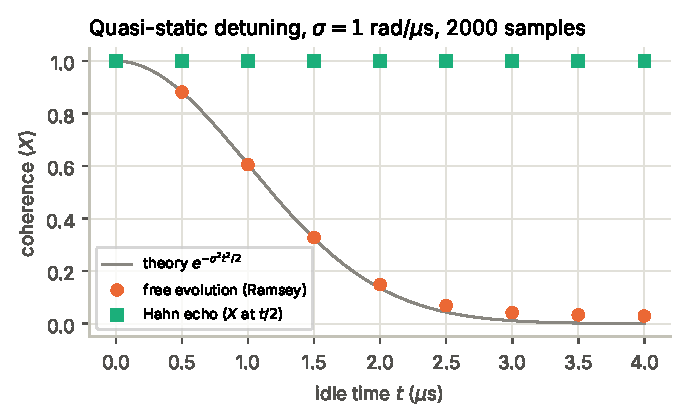
\includegraphics[width=\textwidth]{dd}
    \end{column}
    \begin{column}{0.40\textwidth}
      \small
      CUDA-Q (\texttt{qpp-cpu}): average of $\langle X\rangle$ over 2000 random detunings.
      \begin{itemize}\itemsep1pt\scriptsize
        \item free evolution follows $e^{-\sigma^2t^2/2}$ (at $t = 2\,\mu$s: \numddfree{}; theory \numddtheory; Monte-Carlo error $\approx\pm0.02$)
        \item the echo restores $\langle X\rangle = \numddecho$ exactly
        \item real noise has a spectrum: DD filters the slow part
      \end{itemize}
    \end{column}
  \end{columns}
\end{frame}

\begin{frame}[label=fQEC]{Quantum error correction fundamentals}
  \begin{columns}[T]
    \begin{column}{0.52\textwidth}
      \small
      \key{3-qubit bit-flip code}: $\alpha\ket0 + \beta\ket1 \mapsto \alpha\ket{000} + \beta\ket{111}$; measure the parities $Z_0Z_1$, $Z_1Z_2$ (syndrome); flip the
      indicated qubit.
      \begin{center}
      \begin{quantikz}[row sep=0.15cm, column sep=0.25cm]
        \lstick{$\ket\psi$} & \ctrl{1} & \ctrl{2} & \gate[3,style={fill=qorange!15}]{X\text{ w.p. }p} & \ctrl{1} & \ctrl{2} & \targ{} & \qw\\
        \lstick{$\ket0$} & \targ{} & \qw & & \targ{} & \qw & \ctrl{-1} & \qw\\
        \lstick{$\ket0$} & \qw & \targ{} & & \qw & \targ{} & \ctrl{-1} & \qw
      \end{quantikz}
      \end{center}
      \scriptsize encode \quad noise \quad decode + majority vote (Toffoli)
    \end{column}
    \begin{column}{0.44\textwidth}
      \small
      Logical error $P_L = 3p^2 - 2p^3$:
      \begin{itemize}\itemsep1pt\scriptsize
        \item $p = 0.1$: $P_L = 0.028$; $p = 0.01$: $P_L = 0.0003$
        \item better than a bare qubit iff $p < \frac12$
        \item protects only against $X$; Shor's 9-qubit code and surface codes protect against all Pauli errors
      \end{itemize}
      \key{Surface codes}: $p_L \approx A(p/p_{\text{th}})^{(d+1)/2}$, threshold $p_{\text{th}} \sim 1\,\%$; $d = 3 \to 5$ at $p/p_{\text{th}} = 0.1$ gains a factor 10.
      \tagtheory
    \end{column}
  \end{columns}
\end{frame}

\begin{frame}[label=fQECfig]{The bit-flip code, simulated \tagillus}
  \begin{columns}[T]
    \begin{column}{0.52\textwidth}
      \centering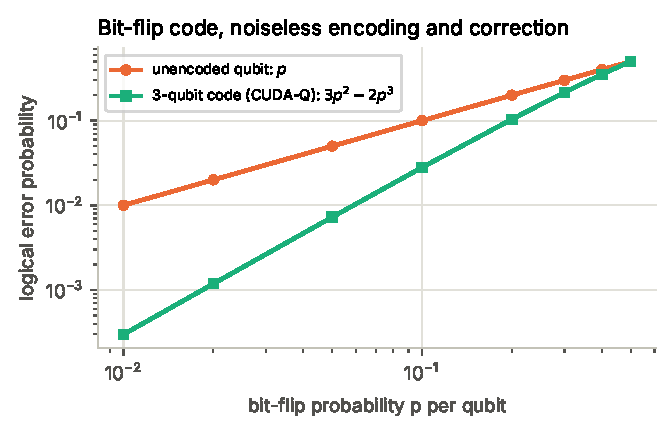
\includegraphics[width=\textwidth]{qec}
    \end{column}
    \begin{column}{0.44\textwidth}
      \small
      CUDA-Q density matrix: bit-flip channel on identity gates (\texttt{rx(idle)}) after encoding; noiseless decoding.
      \begin{itemize}\itemsep1pt\scriptsize
        \item matches $3p^2 - 2p^3$ to \numqeccheck
        \item $p = 0.01$: \numqecone; $p = 0.1$: \numqecten
        \item idealised: perfect gates and syndrome extraction. With noisy gates a fault-tolerant design and a threshold are needed.
      \end{itemize}
    \end{column}
  \end{columns}
\end{frame}

\begin{frame}[label=fTwirl]{Twirling: turning coherent errors into Pauli noise \tagtheory}
  \begin{columns}[T]
    \begin{column}{0.52\textwidth}
      \small
      Insert a random Pauli $P$ before a gate $G$ and the compensating $P' = GPG^\dagger$ after it (for Clifford $G$, $P'$ is again a Pauli):
      the ideal circuit is unchanged. Averaging over random compilations,
      \[ \E_{\text{twirled}}(\rho) = \tfrac{1}{4}\textstyle\sum_PP^\dagger\E(P\rho P^\dagger)P \]
      is a \key{Pauli channel} with the same average fidelity.
    \end{column}
    \begin{column}{0.44\textwidth}
      \begin{block}{Why it matters}
        \scriptsize
        \begin{itemize}\itemsep1pt
          \item coherent errors stop adding in amplitude (Part 1: $0.995$ vs.\ $0.036$)
          \item makes Pauli noise models --- like the notebook's --- realistic
          \item basis of probabilistic error cancellation and of RB's interpretation
        \end{itemize}
      \end{block}
    \end{column}
  \end{columns}
\end{frame}

\begin{frame}[label=fHW]{Simulated noise versus hardware noise}
  \begin{columns}[T]
    \begin{column}{0.5\textwidth}
      \small \key{What simple noise models miss}
      \begin{itemize}\itemsep1pt\scriptsize
        \item \key{correlated} and \key{crosstalk} errors between neighbouring qubits
        \item \key{non-Markovian} noise (memory, $1/f$ spectra), drift over hours
        \item \key{leakage} out of the qubit subspace
        \item idle-qubit errors while others are being gated (the notebook adds noise only after gates)
        \item readout errors, state-preparation errors
        \item device-specific connectivity (extra SWAPs)
      \end{itemize}
    \end{column}
    \begin{column}{0.46\textwidth}
      \begin{block}{Good practice}
        \scriptsize calibrate a model from device data ($T_1$, $T_2$, RB/IRB rates, readout matrices), validate it against small hardware experiments, and report
        simulation and hardware results separately.
      \end{block}
      \begin{alertblock}{In this lecture}
        \scriptsize every number is a simulation on a CPU; nothing was run on a quantum processor.
      \end{alertblock}
    \end{column}
  \end{columns}
\end{frame}

\begin{frame}[label=fFuture]{Hardware noise considerations and future directions}
  \begin{columns}[T]
    \begin{column}{0.5\textwidth}
      \small
      \begin{itemize}\itemsep2pt
        \item gate errors around $10^{-3}$ (two-qubit) and below on leading platforms; QEC below threshold demonstrated on small surface codes
        \item noise-aware compilation: mapping, scheduling, DD insertion
        \item learning noise models (Pauli-noise learning, cycle benchmarking)
        \item scalable simulation: GPU trajectories, tensor networks, stabilizer + few non-Clifford gates
        \item from mitigation to logical qubits
      \end{itemize}
    \end{column}
    \begin{column}{0.46\textwidth}
      \begin{block}{Natural extensions of \texttt{Noise\_Simulation.ipynb}}
        \scriptsize
        \begin{itemize}\itemsep1pt
          \item readout-error channel and its mitigation
          \item idle noise from $T_1$, $T_2$ and gate durations
          \item noise models for the other notebooks' circuits (QFT, QAOA, VQE)
          \item GPU trajectory runs at 20--30 qubits; ZNE
        \end{itemize}
      \end{block}
    \end{column}
  \end{columns}
\end{frame}

\begin{frame}[label=fTry]{Try it yourself: \texttt{Noise\_Simulation.ipynb}}
  \begin{columns}[T]
    \begin{column}{0.5\textwidth}
      \small Edit only Section 3:
      \begin{itemize}\itemsep1pt\scriptsize
        \item \texttt{NOISE\_MODEL = "phase\_flip"}: population stays 1, parity collapses
        \item \texttt{N\_QUBITS = 100}: \texttt{stim} still runs in seconds; fidelity at fixed $p$ falls faster
        \item \texttt{SIMULATION\_METHOD = "density\_matrix"}, \texttt{N\_QUBITS = 8}: state fidelity and purity
        \item \texttt{NOISE\_MODEL = "amplitude\_damping"}: outcomes biased towards 0
        \item \texttt{CIRCUIT = "mirror"}, \texttt{N\_QUBITS = 6}: a non-Clifford benchmark
      \end{itemize}
    \end{column}
    \begin{column}{0.46\textwidth}
      \small Reproduce these slides:
      \begin{itemize}\itemsep1pt\scriptsize
        \item \texttt{cd presentations/noise\_source}
        \item \texttt{python make\_figures.py} (re-executes the notebook's sweep and all experiments, $\sim5$ min)
        \item \texttt{latexmk -pdf noise\_lecture.tex}
      \end{itemize}
      Test yourself: \texttt{assessments/Noise\_Question\_Paper.pdf} (80 questions) and the separate Answer Book.
    \end{column}
  \end{columns}
\end{frame}

% =====================================================================================
\section{Practice and summary}
\begin{frame}{Exercises}
  \begin{enumerate}\small
    \item Find the Bloch vector and purity of $\rho = \begin{psmallmatrix}0.6 & 0.2i\\ -0.2i & 0.4\end{psmallmatrix}$.
    \item Apply amplitude damping with $\gamma = 0.5$ to $\ket1$ and to $\ket+$.
    \item Show that the phase-flip channel with $p$ equals phase damping with $\lambda = 4p(1-p)$.
    \item A depolarizing channel (CUDA-Q) with $p = 0.06$ acts twice. Give the single equivalent $p$.
    \item $T_1 = 120\,\mu$s, $T_2 = 90\,\mu$s. Find $T_\varphi$ and the coherence of $\ket+$ after $30\,\mu$s.
    \item No-error probability of the notebook's 20-qubit GHZ circuit with depolarizing $p = 0.005$.
    \item ZNE gives $E(1) = 0.70$, $E(2) = 0.52$, $E(3) = 0.40$. Linear and Richardson estimates?
    \item 3-qubit bit-flip code at $p = 0.05$: logical error?
  \end{enumerate}
\end{frame}

\begin{frame}{Answers}
  \small
  \begin{enumerate}
    \item $r_z = 0.2$, $\rho_{10} = -0.2i = \frac{r_x + ir_y}{2} \Rightarrow r_y = -0.4$: $\vec r = (0, -0.4, 0.2)$; purity $\frac{1 + 0.2}{2} = 0.6$.
    \item $\ket1 \mapsto \operatorname{diag}(0.5, 0.5)$; $\ket+ \mapsto \begin{psmallmatrix}0.75 & 0.354\\ 0.354 & 0.25\end{psmallmatrix}$ ($\frac{\sqrt{0.5}}{2} = 0.354$).
    \item Coherence factors: $1 - 2p = \sqrt{1-\lambda} \Rightarrow \lambda = 1 - (1-2p)^2 = 4p(1-p)$.
    \item $(1 - 0.08)^2 = 0.8464 = 1 - \frac{4p}{3} \Rightarrow p = 0.1152$.
    \item $\frac1{T_\varphi} = \frac1{90} - \frac1{240} = 0.006944 \Rightarrow T_\varphi = 144\,\mu$s; $|\rho_{01}| = \frac12e^{-30/90} = 0.358$.
    \item $G = 1 + 19 = 20$: $0.995^{20} = 0.905$.
    \item Linear $2(0.70) - 0.52 = 0.88$; Richardson $3(0.70) - 3(0.52) + 0.40 = 0.94$.
    \item $3(0.05)^2 - 2(0.05)^3 = 0.0075 - 0.00025 = 0.00725$.
  \end{enumerate}
\end{frame}

\begin{frame}{Summary}
  \begin{columns}[T]
    \begin{column}{0.56\textwidth}
      \footnotesize
      \begin{itemize}\itemsep1pt
        \item Noise turns pure states into mixed states: density matrices, Bloch ball, purity, fidelity.
        \item Channels: $\E(\rho) = \sum K\rho K^\dagger$, $\sum K^\dagger K = I$ (CPTP); Kraus sets are not unique.
        \item Bit/phase/bit-phase flip and depolarizing shrink the ball; amplitude damping also shifts it ($T_1$); phase damping $\leftrightarrow T_\varphi$; $\frac1{T_2} = \frac1{2T_1} + \frac1{T_\varphi}$.
        \item Coherent errors accumulate quadratically, stochastic ones linearly; readout errors are classical.
        \item CUDA-Q: \texttt{NoiseModel} + \texttt{stim} / density matrix / trajectories; the notebook's GHZ sweep reproduced exactly.
        \item Mitigation (ZNE, readout, DD) estimates or suppresses; only QEC protects the state; simulation predicts.
      \end{itemize}
    \end{column}
    \begin{column}{0.40\textwidth}
      \begin{block}{Further reading}
        \scriptsize
        \begin{itemize}\itemsep0pt
          \item M.\ Nielsen, I.\ Chuang, \emph{Quantum Computation and Quantum Information}, Ch.~8 and 10
          \item J.\ Preskill, \emph{Lecture notes for Physics 219}, Ch.~3
          \item K.\ Temme, S.\ Bravyi, J.\ Gambetta, \emph{Error mitigation for short-depth circuits}, PRL 119 (2017)
          \item P.\ Krantz et al., \emph{A quantum engineer's guide to superconducting qubits}, APR 6 (2019)
          \item NVIDIA CUDA-Q documentation: noise modelling
          \item This repository: \texttt{Noise\_Simulation.ipynb}, \texttt{assessments/Noise\_*.pdf}
        \end{itemize}
      \end{block}
    \end{column}
  \end{columns}
\end{frame}

% =====================================================================================
\section{Syllabus map}
\begin{frame}{Syllabus coverage: topics 1--40}
  \tiny
  \begin{columns}[T]
    \begin{column}{0.49\textwidth}
\resizebox{\linewidth}{!}{\begin{tabular}{rlr}\toprule \# & topic & slides\\ \midrule
1 & Introduction to ideal quantum computing & \pageref{fIdeal} \\
2 & Ideal versus noisy circuits & \pageref{fIdealNoisy}, \pageref{fRec} \\
3 & Sources of quantum noise & \pageref{fSources} \\
4 & Decoherence & \pageref{fDecoh} \\
5 & Quantum state fidelity & \pageref{fFid} \\
6 & Gates and imperfect operations & \pageref{fImperfect} \\
7 & Bit-flip errors & \pageref{fBF} \\
8 & Phase-flip errors & \pageref{fPF} \\
9 & Bit-phase-flip errors & \pageref{fYF} \\
10 & Depolarizing noise & \pageref{fDep} \\
11 & Amplitude damping & \pageref{fAD} \\
12 & Phase damping & \pageref{fPD} \\
13 & Amplitude vs phase damping & \pageref{fADPD} \\
14 & Quantum channels & \pageref{fChan} \\
15 & Kraus operators & \pageref{fChan}, \pageref{fCPTP} \\
16 & Density matrices & \pageref{fDM} \\
17 & Pure and mixed states & \pageref{fPure} \\
18 & CPTP maps & \pageref{fCPTP} \\
19 & Single-qubit noise models & \pageref{fSingle}, \pageref{fBlochCh} \\
20 & Two-qubit gate noise & \pageref{fTwoQ} \\
\bottomrule\end{tabular}}
    \end{column}
    \begin{column}{0.49\textwidth}
\resizebox{\linewidth}{!}{\begin{tabular}{rlr}\toprule \# & topic & slides\\ \midrule
21 & Measurement errors & \pageref{fReadout} \\
22 & Readout noise & \pageref{fReadout}, \pageref{fROM} \\
23 & Thermal relaxation & \pageref{fT1T2}, \pageref{fT1T2fig} \\
24 & $T_1$ and $T_2$ times & \pageref{fT1T2}, \pageref{fT1T2fig} \\
25 & Noise channels and circuit execution & \pageref{fExec} \\
26 & Noise injection in simulation & \pageref{fInject}, \pageref{fPitfalls} \\
27 & Shot-based simulation & \pageref{fShots} \\
28 & Noisy vs noiseless execution & \pageref{fNoisyVs}, \pageref{fKinds} \\
29 & State and process fidelity & \pageref{fFid}, \pageref{fRates}, \pageref{fDMres} \\
30 & Error rates and gate errors & \pageref{fRates} \\
31 & Noise simulation using CUDA-Q & \pageref{fInject}, \pageref{fMethods} \\
32 & Repository walkthrough & \pageref{fStruct}, \pageref{fModel}, \pageref{fKernels}, \pageref{fAuto}, \pageref{fGlance} \\
33 & Noise on QFT, VQE, QAOA & \pageref{fAlgs} \\
34 & Noise benchmarking & \pageref{fRec}, \pageref{fScale} \\
35 & Error mitigation & \pageref{fMitig} \\
36 & Zero-noise extrapolation & \pageref{fZNE}, \pageref{fZNEfig} \\
37 & Readout-error mitigation & \pageref{fROM} \\
38 & Dynamical decoupling & \pageref{fDD}, \pageref{fDDfig} \\
39 & Error-correction fundamentals & \pageref{fQEC}, \pageref{fQECfig} \\
40 & Hardware noise, future directions & \pageref{fHW}, \pageref{fFuture} \\
\bottomrule\end{tabular}}
    \end{column}
  \end{columns}
\end{frame}
\end{document}
